% $Id: template.tex 11 2007-04-03 22:25:53Z jpeltier $

\documentclass{vgtc}                          % final (conference style)
% \documentclass[review]{vgtc}                 % review
%\documentclass[widereview]{vgtc}             % wide-spaced review
%\documentclass[preprint]{vgtc}               % preprint
%\documentclass[electronic]{vgtc}             % electronic version

%% Uncomment one of the lines above depending on where your paper is
%% in the conference process. ``review'' and ``widereview'' are for review
%% submission, ``preprint'' is for pre-publication, and the final version
%% doesn't use a specific qualifier. Further, ``electronic'' includes
%% hyperreferences for more convenient online viewing.

%% Please use one of the ``review'' options in combination with the
%% assigned online id (see below) ONLY if your paper uses a double blind
%% review process. Some conferences, like IEEE Vis and InfoVis, have NOT
%% in the past.

%% Figures should be in CMYK or Grey scale format, otherwise, colour 
%% shifting may occur during the printing process.

%% it is recommended to use ``\cref{sec:bla}'' instead of ``Fig.~\ref{sec:bla}''
\graphicspath{{figs/}{figures/}{pictures/}{images/}{./}} % where to search for the images

\usepackage{times}                     % we use Times as the main font
\renewcommand*\ttdefault{txtt}         % a nicer typewriter font

%% Only used in the template examples. You can remove these lines.
\usepackage{booktabs}                  % only used for the table example
\usepackage{lipsum}                    % used to generate placeholder text
\usepackage{mwe}                       % used to generate placeholder figures

%% We encourage the use of mathptmx for consistent usage of times font
%% throughout the proceedings. However, if you encounter conflicts
%% with other math-related packages, you may want to disable it.
\usepackage{mathptmx}                  % use matching math font
\usepackage{amsmath}                   % for \genfrac and advanced math


%% If you are submitting a paper to a conference for review with a double
%% blind reviewing process, please replace the value ``0'' below with your
%% OnlineID. Otherwise, you may safely leave it at ``0''.
\onlineid{0}

%% declare the category of your paper, only shown in review mode
\vgtccategory{Research}

%% allow for this line if you want the electronic option to work properly
\vgtcinsertpkg

%% In preprint mode you may define your own headline. If not, the default IEEE copyright message will appear in preprint mode.
%\preprinttext{To appear in an IEEE VGTC sponsored conference.}

%% This adds a link to the version of the paper on IEEEXplore
%% Uncomment this line when you produce a preprint version of the article 
%% after the article receives a DOI for the paper from IEEE
%\ieeedoi{xx.xxxx/TVCG.201x.xxxxxxx}


%% Paper title.

\title{ImproVisAR: Designing Augmented Reality \\Piano Roll for Teaching Improvisation}

%% This is how authors are specified in the conference style

%% Author and Affiliation (single author).
%%\author{Roy G. Biv\thanks{e-mail: roy.g.biv@aol.com}}
%%\affiliation{\scriptsize Allied Widgets Research}

%% Author and Affiliation (multiple authors with single affiliations).
%%\author{Roy G. Biv\thanks{e-mail: roy.g.biv@aol.com} %
%%\and Ed Grimley\thanks{e-mail:ed.grimley@aol.com} %
%%\and Martha Stewart\thanks{e-mail:martha.stewart@marthastewart.com}}
%%\affiliation{\scriptsize Martha Stewart Enterprises \\ Microsoft Research}

%% Author and Affiliation (multiple authors with multiple affiliations)
\author{
Jordan Aiko Deja\thanks{e-mail: jordan.deja@dlsu.edu.ph}\\
\scriptsize De La Salle University, Philippines
\and
Sandi Štor\thanks{e-mail: sandistor@gmail.com}\\
\scriptsize JazzObala, Portorož, Slovenia
\and
Ilonka Pucihar\\
\scriptsize University of Ljubljana, Slovenia
\and
Maheshya Weerasinghe\thanks{e-mail: maheshya.weerasinghe@famnit.upr.si}\\
\scriptsize University of Primorska, Slovenia
\and
Klen Čopič Pucihar\thanks{e-mail: klen.copic@famnit.upr.si}\\
\scriptsize University of Primorska, Slovenia
\and
Matjaž Kljun\thanks{e-mail: matjaz.kljun@upr.si}\\
\scriptsize University of Primorska, Slovenia
}

%% A teaser figure can be included as follows
\teaser{
  \centering
  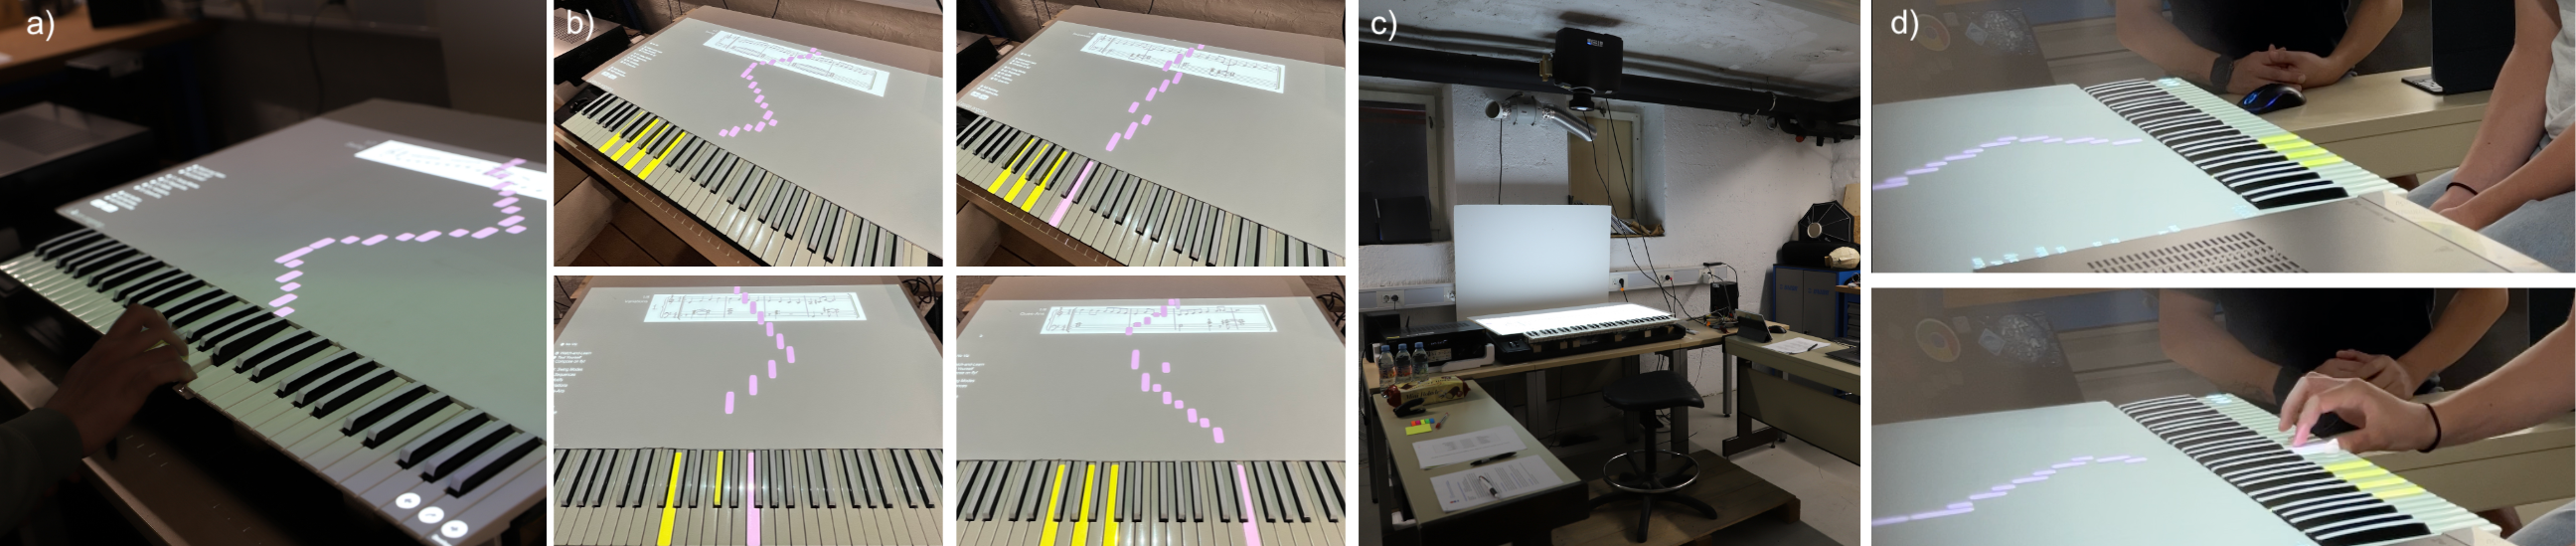
\includegraphics[width=\linewidth]{figs/ieeevrteaser.png}
  \caption{%
  	In \textit{ImproVisAR}, a) falling piano roll is shown to the user to help them map music sheets with keypress. b) Lessons on improvisation along with harmony play along are projected showing all modes in swing, sequences, variations and question-and-answer. c) Our interface setup having a projector overlaying projections on top of a white surface as an extended part of a modified keyboard. d) Action photos of a (top) student being shown how to play the lesson and (bottom) trying the lesson during our \texttt{Try Yourself} mode.  %
  }
  \label{fig:teaser}
}

%% Abstract section.
\abstract{%
Improvisation is an important skill of music instrument learning in general, but still a less-taught topic in traditional piano learning. To improvise properly, one must have an adequate music vocabulary, subjective confidence, and be comfortable in performing. This makes teaching piano improvisation a challenge where technology intervention could be beneficial. Prior short-term studies on augmented piano roll visualisations have shown an impact in teaching sight-reading and finger-hand-arm-body movement for novice students. However, how a similar approach can benefit advanced students in long-term learning and encouraging complex music concepts such as improvisation remains under-explored. To address this gap, we present \textit{ImproVisAR}, an interactive piano training system that teaches improvisation using augmented piano roll visualisations. Improvisation concepts and tools derived through a co-design process with experts are presented as learning modes, which aim to equip learners with enough context enabling them to improvise when performing. Findings from a pilot ($n=6$) show the potential of the tool in reducing cognitive load and improving user experience during learning. We also conducted an initial study ($n=2$) where participants tried all lessons and modes in-depth. Lastly, we discuss these findings towards a controlled longitudinal study which aims to fully explore the effects of teaching piano improvisation with our system. %to learned pianists. 
%
}

%% Keywords that describe your work. Will show as 'Index Terms' in journal
%% please capitalize first letter and insert punctuation after last keyword.
\keywords{piano, jazz, improvisation, augmented reality, piano roll, visualisation}

%% Copyright space is enabled by default as required by guidelines.
%% It is disabled by the 'review' option or via the following command:
% \nocopyrightspace

%%%%%%%%%%%%%%%%%%%%%%%%%%%%%%%%%%%%%%%%%%%%%%%%%%%%%%%%%%%%%%%%
%%%%%%%%%%%%%%%%%%%%%% START OF THE PAPER %%%%%%%%%%%%%%%%%%%%%%
%%%%%%%%%%%%%%%%%%%%%%%%%%%%%%%%%%%%%%%%%%%%%%%%%%%%%%%%%%%%%%%%%

\begin{document}

%% The ``\maketitle'' command must be the first command after the
%% ``\begin{document}'' command. It prepares and prints the title block.

%% the only exception to this rule is the \firstsection command
\firstsection{Introduction}

\maketitle

%% \section{Introduction} %for journal use above \firstsection{..} instead
\par Learning improvisation is an important component in music learning. Yet, it often receives less emphasis compared to other skills such as body synchronisation and sight-reading~\cite{deja2021encouraging}. This is due to several factors, such as the subjective nature of improvisation and creativity, the needed time to learn the basics of finger-to-hand-to-arm movement, core music theory and others. Evaluating improvisation in the learning setting is also challenging due to the same subjective elements. According to piano teaching experts~\cite{deja2022survey} improvisation is a skill that learners should learn at all levels; however, it is usually practised only by advanced learners. For them, showcasing improvisational skills indicates a comprehensive musical understanding and broader knowledge of the musical vocabulary. Piano teaching experts also note that improvisation fosters creativity in learners and performers of all levels. Thus, teaching improvisation to beginners and experienced players improves rhythmic precision, reading music, focus, self-analysis, creativity, and confidence~\cite{chyu2004teaching, burnard2000children, allen2013free}.


%Improvisation in the piano, a crucial skill in music, often does not get enough attention in traditional piano teaching methods~\cite{deja2021encouraging}. 

\par Through the years, several works and approaches have been introduced to make piano learning easier and more accessible. One of them is the use of digital augmentations such as the use of projected holograms~\cite{xiao2010mirrorfugue, xiao2011duet, cai2019designa, gerry2019adept}, hand tracking visualisations~\cite{barakonyi2005augmented, huang2011piano}, animated avatars and agents~\cite{fernandez2016piano, xiao2014andante} and falling piano roll visualisations~\cite{weing2013piano, takegawa2012piano, rogers2014piano, birhanu2017keynvision}. It is well-established that employing these digital augmentations can effectively teach musical concepts such as coordinating hands, fingers, and arms~\cite{barakonyi2005augmented}, boost motivation~\cite{rogers2014piano, montano1984effect}, and aid in sight-reading~\cite{chiang2015oncall, schmalstieg2007experiences, yang2012augmented, yang2013visual}. However, to the best of our knowledge, none of these augmentations and techniques have been used to teach advanced topics such as improvisations as well as advanced learners in longitudinal settings~\cite{deja2022survey}. 

\par Various augmented piano prototypes have to some extent facilitated improvisation through diverse approaches and functionalities. A prevalent strategy involves integrating gesture detection, enabling musicians to utilize their hands more freely during performances, thereby enriching their musical vocabulary~\cite{schmalstieg2007experiences, mcpherson2010augmenting, mcpherson2010toward, sandnes2019enhanced, das2017music}. Certain prototypes have empowered users to execute natural gestures, allowing for more creative expression~\cite{karolus2020hit, granieri2019reach, ogata2017keyboard}. These studies have explored various aspects, including levels of expressiveness and improvisation, revealing that the additional finger-based controls do not disrupt performers' playing flow. Researchers suggest that improvisation enhances user experience, particularly in live settings, as evidenced by several prototype implementations~\cite{nicolls2012gesturally, xiao2013mirrorfugue, das2017music, santiniaugmented}. Moreover, in certain cases, improvisation has been instrumental in enhancing sound quality, thereby impacting not only performers but also listeners~\cite{dahlstedt2015mapping, yang2012augmented, yang2013visual}. Generally, these works have enabled improvisation through other diverse techniques that encourage a more free flow and creative experience. However, mastering improvisation is akin to mastering a language where one must be familiar with the rules, context and tools along with continued practice. While existing prototypes enable to support the act of improvisation in the piano, none of these works have attempted to teach improvisation as a skill to learners. 

\par To address this gap, we introduce an augmented reality (AR) piano  training system for jazz improvisation, named \textit{ImproVisAR}. We describe the key features of its interface, which incorporates piano roll visualisations, organised into lessons and modes developed with the experts' input, with the primary aim of facilitating the teaching of piano improvisation. We also present the findings from (i) a pilot study ($n=6$) that assessed subjective cognitive load and perceived user experience while using a selection of lessons and the system, and (ii) an initial study ($n=2$) where learners completed the entire learning experience. The findings show that piano roll visualisations in \textit{ImproVisAR} are effective also for teaching advanced learners complex music concepts such as jazz improvisation, and that the prototype is prepared for a longitudinal study. 

%there is a gap in exploring how augmentation can encourage piano and other instrument users to improvise, as noted in recent research. 

%To properly assess this potential, it's vital to understand how to design augmented reality (AR) training systems for teaching improvisation. Given the limited research on piano augmentations for improvisation, involving piano teachers in the design process can aid in crafting a training system tailored for this purpose. Drawing from previous studies on co-designing musical instruments and interfaces, we can apply principles and techniques to guide this process effectively.
%\par In summary, this paper presents the following contributions: a) \textbf{narratives from our co-design process of an AR training system for piano improvisation} and its features, which we refer to as \textit{ImproVISe}, and b) \textbf{guidelines and recommendations} to address challenges in assessing piano improvisation in the context of learning.

\section{Background and Related Work}
\label{sec:rrl}
\par Piano, besides violin, is a popular instrument among novice learners starting out in music~\cite{ericsson1993role}. It is thus not surprising that it is among most digitally augmented instrument~\cite{deja2022piano}. In this section %In positioning our contribution, 
we look at the current state-of-the-art of %where and how 
piano augmentations in general and % have been used in learning. Since we also focus our contribution on improvisation which is a least-explored area both in piano didactics and piano augmentation, we also look at the latest approaches in piano augmentation 
in the context of improvisation. % (e.g. teaching, learning, collaborating). 
We also borrow from existing approaches that have worked on both piano training systems~\cite{deja2022survey} and augmented reality training systems~\cite{santos2013augmented} considering different learning modes, lesson delivery features and other augmentations. 
% \subsection{Augmented Pianos on Improvisation}
% \subsection{Piano Roll Visualisations}

%jazz improvisation and other genres? 
\subsection{Piano Roll Visualisations in Piano Learning}

\par Research has shown that the complexity of traditional music notation, particularly in advanced pieces, increases the cognitive load, %experienced by piano  
highlighting the need for simpler representations. Piano roll visualisation, or simply animated falling bars, is one of the most widely used techniques in digital piano augmentation~\cite{deja2022survey}. By simplifying complex music sheet notation into animated falling bars, users can easily understand what keys to press and the precise timing for pressing and releasing them. This technique has proven effective in teaching novice users sight-reading and finger-hand body synchronisation. %This way, learners can focus on practising different song pieces and be familiar with how concepts such as tempo and melody can be visualised and simplified to the novice learner.
Given that sight-reading is a crucial yet challenging skill for piano playing, this approach is particularly valuable. Several prototypes have addressed the sight-reading challenges using piano roll visualisation~\cite{rogers2014piano, birhanu2017keynvision, sun2018mr, cai2019designb, weing2013piano, rogers2014piano}, overlaying visual cues directly on top of the piano either through projections, see-through mixed reality or virtual reality environments. Piano roll visualisations have been found to reduce cognitive load, providing novices with better opportunities to learn musical pieces. 

\par A recent survey~\cite{deja2022survey} suggests that an ideal augmented prototype should integrate sheet notation into visually engaging representations that aid learners process the information, rather than removing it. Only few systems have combined piano roll visualisations with music sheet notations~\cite{takegawa2012piano, yang2012augmented, yang2013visual}. This approach aims to blend conventional methods with visual elements, enhancing the overall piano learning experience and make it more enjoyable. %In designing  \textit{ImproVisAR}, we follow the similar approach where we provide music notation for learners to use as reference and have falling piano roll bars that visualise the same music sheets. 
The survey authors also emphasised that audio feedback should complement the visual augmentation, especially when dealing with complex chords and progressions, which current prototypes do not encompasses. %Specifically, our design of \textit{ImproVisAR} also employs this approach by introducing the \texttt{Watch-and-Listen} mode which will be described in the next section. 

\par One of the few prototypes using piano roll visualisations to teach piano improvisation is Music Everywhere~\cite{das2017music}. While this work presents the features of the systems, it provides limited findings into the impact on the improvisation itself. 
The system involved displaying highlighted bars that users could press during a play-along band performance in a mixed reality environment. Additionally, the system used reverse piano roll visualisations (rising bars instead of falling) to help users review what they had improvised in real-time. 

\par Our work builds on these foundation by: (i) emphasising both music sheets and visualisations, (ii) providing audio feedback complementing visual augmentations, and (iii) and by meticulously designing the learning content that can be used in controlled studies for future research. 

%Some works have removed the traditional music sheet notation entirely while some chose to keep them. For the former, They argue that  Then there are systems that chose to use both falling piano roll bars and their corresponding mapping with traditional music sheets. They have shown that both music sheets along with falling piano roll visualisations, allow learners to map complex notation with bars . 

\subsection{Augmented Pianos and Improvisation}

\par In addition to piano roll visualisations, other digital methods have been developed to assist in piano learning. When focusing on improvisation,  techniques have ranged from using a keyboard pitch wheel interface to encourage playfullness during improvisation~\cite{kastner2014exploring}, displaying hologramic music sheets and highlighting possible keys for pressing on an existing melody~\cite{uddin2021image, sandnes2019enhanced}, to employing tracking sensors to detect gestures that can enhance expressiveness during performances~\cite{gordon2011roots, dahlstedt2015mapping, mcpherson2015buttons, montano1984effect, newton2011examining}. These works have explored various aspects of piano improvisation, such as composing, performing and recording~\cite{deja2022vision}. 

\par %Since piano improvisation builds on being able to compose on the fly and at the same time being able to confidently-perform, the skill involves looking beyond body-hand-finger synchronisation and reading music sheet notation, but rather having the confidence to play around with notes, is an also an essential part of the process. As we know, being able to improvise has been observed to 
Piano improvisation involves not just body-hand-finger synchronisation and reading music notation, but also the confidence to experiment with notes. This skill is crucial, as improvisation has been shown to improve rhythmic accuracy and note-reading abilities to improve rhythmic accuracy and note-reading skills~\cite{montano1984effect}. 
%Most of these prior works have explored piano improvisation focusing on supporting performance, specifically, from the perspective of knowing how to move while improvising (e.g. gesture detection~\cite{granieri2019reach}, such as by-swinging and playing along with a given melody~\cite{karolus2020hit, ogata2017keyboard}). There are also several studies where they have observed varying levels of expressiveness or performances during piano improvisation performances~\cite{das2017music, nicolls2010seeking, santiniaugmented, xiao2013mirrorfugue} but not specifically on supporting the actual composition process during an improvisation task. They focused their augmentations on supporting a continuous flow during performances which improves the usages of their current musical vocabulary~\cite{mcpherson2010augmenting, mcpherson2010toward, sandnes2019enhanced, schmalstieg2007experiences}. Overall, we know through these studies that improvisation during piano playing generally improves user experiences especially during live performances. 
Previous research has largely focused on supporting performance by helping users move while improvising, such as gesture detection~\cite{granieri2019reach} or playing along with a provided melody~\cite{karolus2020hit, ogata2017keyboard}. Other studies have examined different levels of expressiveness during improvisation performances~\cite{das2017music, nicolls2010seeking, santiniaugmented, xiao2013mirrorfugue}, but these did not specifically address the composition process during improvisation. Instead, their augmentations aimed to support continuous flow during performances, enhancing the use of the performer’s existing musical vocabulary~\cite{mcpherson2010augmenting, mcpherson2010toward, sandnes2019enhanced, schmalstieg2007experiences}. These studies confirm that improvisation generally enhances the user experience, particularly during live performances.

Another type of augmentation %in the piano that has been done to support piano improvisation is by playing around with improving sound quality of produced sounds during performance
to support piano improvisation focuses on improving sound quality during performances~\cite{dahlstedt2015mapping, yang2012augmented, yang2013visual}, %. Their findings have measured improved listener experiences of improvisation performers only. 
with findings showing that these improvements mainly enhanced the listener's experience of the performance.

\par
%Works on actually teaching piano improvisation with the help of digital augmentation is least-explored. We believe that this is due to the subjective nature of improvisation~\cite{laroche2014enacting}, its expressive qualities~\cite{donahue2019piano,xia2017improvised} and having to apply the creative approach in one performance~\cite{solis2009musical, smith1983homer}. However, the task of composing on the fly and assessing the quality of these performances are not well-understood. This research attempts to fill this gap by looking at how our system \textit{ImproVisAR} can be used to actively support and teach improvisation by improving the musical vocabulary of piano performers. We pay particular focus on supporting composing-on-the-fly improvisation, learning it similar to that of the process of learning a language~\cite{deja2024teach} where language is to improvisation as grammar is to scales, motifs, sequences and variations. Thus, in designing the augmentations of \textit{ImproVisAR}, we also look at not just falling piano roll bars but also play-along rhythms, and other audio-based guidance (e.g. having the option to include harmony, adding metronome). 
Despite these prototypes, research on teaching piano improvisation through digital augmentation is limited. This may be due to the subjective nature of improvisation~\cite{laroche2014enacting}, its expressive characteristics~\cite{donahue2019piano,xia2017improvised}, and the challenge of applying creativity in a single performance~\cite{solis2009musical, smith1983homer}. %The process of improvising on the spot and evaluating the quality of these performances remains poorly understood. 
    This study aims to address this gap by exploring how our system, \textit{ImproVisAR}, will actively support and teach improvisation, particularly by expanding the musical vocabulary of piano performers. We focus specifically on supporting real-time composition, approaching it similarly to language learning~\cite{deja2024teach}, where improvisation parallels language, and grammar corresponds to scales, motifs, sequences, and variations. Therefore, in designing the augmentations for \textit{ImproVisAR}, we will incorporate not only falling piano roll bars but also play-along rhythms and other audio-based guidance (e.g., optional harmonies, metronome features).


%These prior works have all looked augmentations in the piano on supporting improvisation through movements, gestures. 

\subsection{Learning Modes and Piano Training Systems}

\par In the context of this paper, we define a learning mode as a system feature that defines how lessons are structured. This affects how learners consume information presented by the augmented reality training system. Much of the successes of augmented piano learning systems can be attributed to a variety of learning modes and features that formed a structure of lesson's content~\cite{deja2022survey}. Key factors in designing these systems typically focus on (i) maintaining learners' motivation~\cite{weing2013piano, rogers2014piano, fernandez2016piano, molloy2019mixed, raymaekers2014game}, (ii) challenging and inspiring learners~\cite{cai2019designb, pan2018pilot}, (iii) tracking individual progress for a more personalised learning experience~\cite{das2017music, rodrigues2021personalization, weing2013piano} or (iv) supplementing traditional classroom instruction by providing additional content to learners~\cite{stryker1997content, chow2013music, guo2021hand, das2017music, stanbury2021holokeys}. 

\par Common learning modes in these systems are the practice mode~\cite{sun2018mr} and the listen-then-reflect mode~\cite{rogers2014piano, weing2013piano}. In practice mode, learners are given a lesson or task to attempt. In a piano training system, this could involve practising a chord~\cite{xiao2013mirrorfugue}, practising a specific song or piece~\cite{schmalstieg2007experiences, mcpherson2013space, pan2018pilot, molero2021novel}, or practising freely within a set time~\cite{takegawa2012piano, weing2013piano, rogers2014piano}. The practise mode has been shown to enhance piano learners' performance, improving their notation accuracy, timing, and overall skill over time. %improvement given a certain period. 

\par The listen-then-reflect mode %usually adds value to the practise mode by taking advantage of both visual and hearing skills of piano learners. 
enhances the practice mode by engaging both the visual and auditory skills of piano learners. In this mode, participants watch and listen to the lesson %and then being given the chance to practice the lesson they just viewed
before practising what they just observed. Systems using this mode~\cite{weing2013piano, rogers2014piano, xiao2014andante} are based on Social Learning Theory (SLT)~\cite{bandura1977social}, %where they follow the attention-retention-reproduction and motivation modes in. 
following the attention, retention, reproduction, and motivation stages. The studies have shown that this mode not only improves learners' performance but %using the training system 
also 
%provided improved levels of motivation and confidence. 
increases their motivation and confidence during the learning process.

Our system, \textit{ImproVisAR}, %considering the successes of these studies and apply SLT in the design of our learning modes which will be described in the next section. 
builds on the success of these studies by applying SLT to our learning modes, as detailed in the next section
%The listen (\textit{attention}) mode in~\cite{rogers2014piano} allows students to hear a piece of music and observe the visualisations, which in \textit{ImproVisAR} is implemented as the \texttt{Watch-and-Listen} mode. The practice (\textit{retention}) mode in~\cite{rogers2014piano} gives students an opportunity to play and receive feedback, which we have implemented as the \texttt{Try Yourself} mode. Lastly, the play (\textit{reproduction and motivation}) mode provides additional feedback, reflected in our \texttt{Test Yourself} and \texttt{Compose-On-The-Fly} modes. While our system does not have an explicitly-dedicated reflect mode, the (\texttt{Try} and \texttt{Test Yourself}) modes offer learners additional opportunities to reflect on their task and performances. 


%In these visualisations, information typically represented in music sheets is condensed into colored bars, which may convey details such as beat length, trills, staccato, among others. 
%According to insights from our interviews,. Additionally, in certain cases, such as with complex chords and progressions, audio feedback may also serve as a beneficial augmentation.

\section{The ImproVisAR System}
\label{sec:system}

\par While building \textit{ImproVisAR} we draw on the recommendations, best practices of augmented pianos and improvisation as described in\autoref{sec:rrl}. We expanded the previous systems with the input from a co-design process with three classical and jazz improvisation teaching experts. The experts designed the music content while in the co-design process the whole system interface was build through several iterations while the system has been tested by the experts, developers and piano students. % as seen in the work of ~\cite{deja2024teach}. 
%In this section, we describe in detail the features of the system from the design and concept of the training system, learning modes, lesson content and other technical features. 
In this section, we provide an in-depth description of the system's features, covering the design and concept of the training system, the learning modes, lesson content, and other technical aspects.

\subsection{Design and Concept}
\label{subsec: design}
\begin{figure*}[tb]% specify a combination of t, b, p, or h for top, bottom, on its own page, or here
  \centering % avoid the use of \begin{center}...\end{center} and use \centering instead (more compact)
  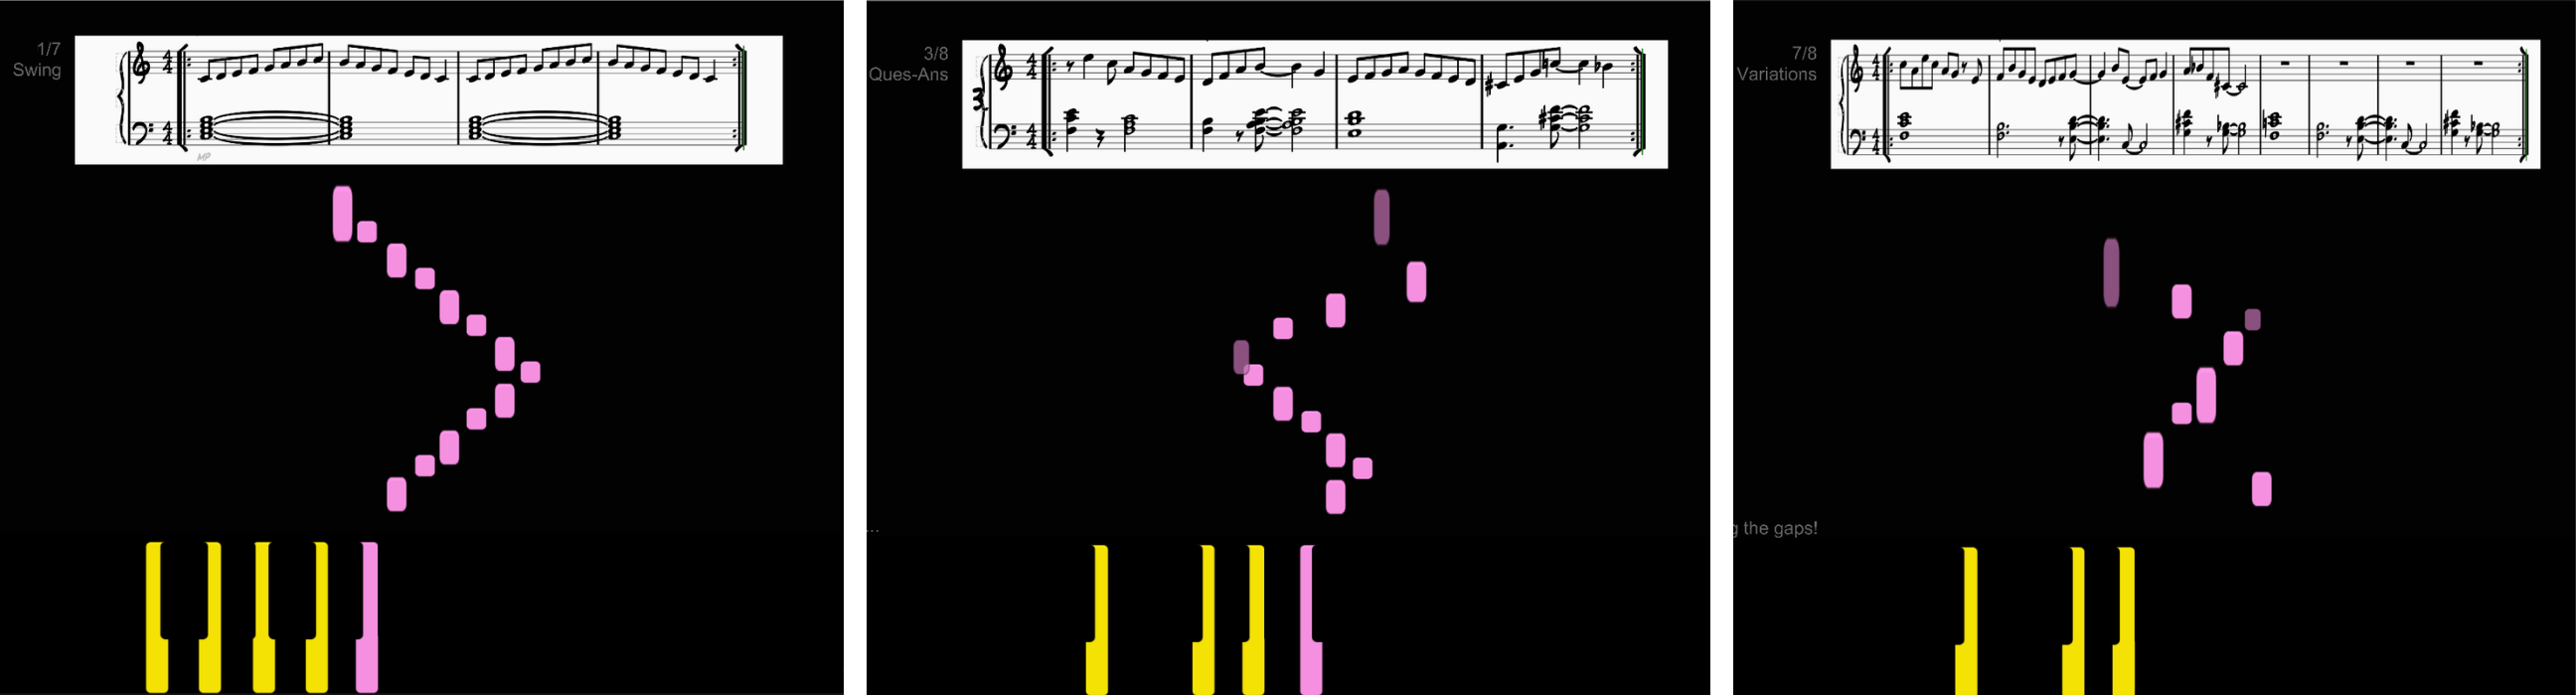
\includegraphics[width=\textwidth]{figs/modes.png}
  \caption{%
  We present several Lessons in different modes. \textbf{(Left)}: Lesson ``01 Swing'' in the \texttt{Watch-and-Listen} mode, where the music sheet for both hands is displayed--melody in pink and harmony in yellow. In the \texttt{Try Yourself} mode, the same visual is shown, but without audio feedback. \textbf{(Middle)}: Lesson ``05 Question-and-Answer'' is also displayed in \texttt{Watch-and-Listen} mode. \textbf{(Right)}: Lesson ``04 Variations'' in the \texttt{Compose-on-the-Fly} mode shows half of the measures as ``blank'', allowing users to improvise. Harmony is played, and the corresponding keys are illuminated, but no piano rolls are used. This enables users to focus on the melody without being influenced by the harmony.   %
  }
  \label{fig:modes}
\end{figure*}

% visualisation features and lessons 
\par Instead of solely relying on sheet music and falling piano roll visualisations, the %\textit{ImproVisAR} system is designed to teach piano improvisation by organising and presenting lessons in a structured way. The 
main objective of the \textit{ImproVisAR} system is to present and organise the different lessons following the Listen-Imitate-Try approach as discussed in~\cite{deja2021encouraging, deja2022survey} and the Attention-Retention-Reproduction-Motivation approach based on SLT~\cite{bandura1977social}. The main interface allows users to select between 3 modes, namely: (i) \texttt{Watch and Listen}, (ii) \texttt{Try Yourself} and (iii) \texttt{Test Yourself}). In each mode users have up to 5 lessons available: Swing, Sequences, Motifs, Variation, and Question and Answer. Users can also select an optional guidance support during the lesson (i.e., metronome, rhythm, harmony), providing an adaptive approach~\cite{deja2021adaptive} to the way they learn. The presented visualisations (and applicable audio feedback) give users a personalised experience based on their selected options. In each particular lesson users can see the upcoming bars moving toward the keyboard, with a portion of the music staff displayed in the upper part of the projected area as seen in \autoref{fig:modes}. When the falling bars align with the keyboard, the corresponding keys are illuminated, signalling to users to press them. Depending on the mode selected, audio feedback may accompany the visual cues. The system supports falling bar visualisations for the right hand (\texttt{G-Clef} staff), while the left-hand staves (\texttt{F-Clef} and \texttt{Clave}) are available as optional guidance in a different format.

%transformation 
\par %The entire system is programmed to simultaneously load multiple files representing the different lessons. % and contents on improvisation. %(N.B. in succeeding paragraphs we refer to improvisation as simply improv). These were provided by our collaborators who are 
%To begin, an improvisatio nlesson is provided in a sibelius \texttt{(.sib)} file which contains the \texttt{G-Clef} which will be used  to generate right-hand visualisations later on. The \texttt{F-Clef} contains musical information on harmonic progress which was the basis of the improvisationcontent taught on all lessons. Generally, we used the \texttt{ii-V-i} and \texttt{ii-V-i-VI} progressions across 4-bars of lessons in the \texttt{C key}. The same \texttt{F-Clef} information is also used to generate play-along harmony audio which the user can toggle if they wish to have harmony support during their lessons. The Claves produce the metronome at a standard \texttt{100 bpm} speed and at $\genfrac{}{}{0pt}{}{4}{4}$ time signature. This is also used to generate background metronome sound effect that users hear across all their lessons. 
The system is designed to simultaneously load multiple files representing different lessons. Each improvisation lesson begins with a Sibelius \texttt{(.sib)} file\footnote{Sibelius - a scorewriter software \url{https://en.wikipedia.org/wiki/Sibelius_(scorewriter)}} that contains the \texttt{G-Clef}, which is used to generate right-hand visualisations. The \texttt{F-Clef} contains harmonic progression information, forming the foundation of the improvisation content in all lessons. We use \texttt{ii-V-i} and \texttt{ii-V-i-VI} progressions across 4-bar lessons in the key of \texttt{C}. This \texttt{F-Clef} data also generates play-along harmony audio, which users can toggle on or off as they prefer. Additionally, the claves provide a metronome set to a standard speed of \texttt{100 bpm} with a $\genfrac{}{}{0pt}{}{4}{4}$ time signature, which plays in the background during all lessons.

\par %At this stage, the provided sibelius file is processed two ways. A \texttt{.mid} file allows the generation of \texttt{MIDI} events which are then used to render the piano roll visualisations. This approach allows us to correctly produce the right pitch at the right time considering the right duration as well. This is then mapped into the 3D space in \texttt{Unity} which are then animated to fall down the piano keys. If audio playback is enabled (e.g. such as in \texttt{Watch-And-Listen} mode which will be explained in \autoref{subsec: modes}) then the same \texttt{.mid} file is also used to generate the sequence of \texttt{MIDIout} events that will be used to produce the right corresponding audio feedback. This gives the impression of having falling bars touch their physical key counterpart (as it is a mixed reality approach) and produce the sound even without pressing the actual keys. This also provides additional room for verification of user press in terms of notation accuracy based on the musical information that is provided in the said \texttt{.mid} file. 
The Sibelius file is processed in two ways. First, it is used to generate a \texttt{.mid} file, which is used to create \texttt{MIDI} events for producing the piano roll visualisations, ensuring the correct pitch, timing, and duration. These visualisations are then mapped in 3D space using \texttt{Unity}, where they are animated to fall onto the piano keys. If audio playback is enabled (e.g., in the \texttt{Watch-And-Listen} mode, described in \autoref{subsec: modes}), the same \texttt{.mid} file generates \texttt{MIDIout} events to produce the corresponding audio feedback. This gives the impression that the falling bars activate their physical key counterpart, even without pressing the keys, providing an additional way to verify notation accuracy based on the musical data in the \texttt{.mid} file.

\par %On the other hand, the same sibelius file is also transformed into a \texttt{musicXML} file which allows us to extract other key musical information that is not usually present in \texttt{.mid} files, which will be useful in generating other music-related assets in our \texttt{Unity} platform. The \texttt{musicXML} file is then exported into the \texttt{abcnotation} which enables the real-time rendering of music sheets in \texttt{Unity} through the use of the \texttt{ABCUnity} API\footnote{\url{https://github.com/matthewcpp/ABCUnity}}. With all these features combined, we are presented with an interface that displays the music sheet notation of the selected lesson, its counterpart falling piano roll visualisation and their respective audio feedback. This interface provides an approach where complex music sheets are mapped with simplified falling bars following prior works. The use of a single file as a source of content ensures that all elements are synchronised together. 
The same Sibelius file is also converted into a \texttt{musicXML} format, allowing us to extract additional musical details that are typically not available in \texttt{.mid} files. This information is useful for generating other music-related assets within our \texttt{Unity} platform. The \texttt{musicXML} file is then exported to \texttt{abcnotation}, which enables real-time music sheet rendering in \texttt{Unity} via the \texttt{ABCUnity} API\footnote{\url{https://github.com/matthewcpp/ABCUnity}}. By integrating these features, the interface presents the music sheet notation of the selected lesson, along with corresponding falling piano roll visualisations and their audio feedback. This setup simplifies complex music sheets by aligning them with falling bars, as seen in previous works, and ensures that all elements are synchronised by using a single file as the content source.

%We present three (3 modes in the system namely (i) Watch and Learn, (ii) Try Yourself and (iii) Test Yourself. Across these three modes, we have five (5) lessons that were organised with the help of our piano teaching experts. These lessons are (a) Learn Swing, (b) Learn Sequences, (c) Learn Motifs, (d) Play with different Variations and (e) Question-Answer. 


%\par The different visualisations projected and animations represent the different lessons and metaphors in piano improvisation. Together with the impro experts, we considered basic concepts such as harmony (specifically \texttt{ii-V-i} and \texttt{ii-V-i-VI} progressions), chord tone soloing (also known as licks), and approaches (e.g., half-step and scale-above). These visualisations were implemented in various lessons (which we refer to as modes) in the system namely \texttt{Guided Press}, \texttt{Rolling Improv}, \texttt{OnWait Roll} and \texttt{Express Press} mode.  

% \subsection{Visualisation Features}

% % features mapped to concepts
% \par The \texttt{Guided Press} mode (\autoref{fig:initprot}B) displays harmonic progressions and chord tones as highlighted keys, allowing users to choose which keys to press~\cite{das2017music}. In yellow, are the keys in the harmonic progression while in pink are the ``musically-correct'' keys that may be pressed for improvisation. In the \texttt{Rolling Improv} mode (\autoref{fig:initprot}C), harmonic progressions appear as falling piano keys in yellow (similar to~\cite{weing2013piano, rogers2014piano}), then revealing chord tones (in pink, like in \texttt{Guided Press} mode) when the right time is triggered. \texttt{OnWait Rolling} mode (\autoref{fig:initprot}D) mirrors \texttt{Rolling Improv} but without the element of timing, allowing the learner to focus on concept absorption without time pressure but with priming~\cite{moro2020performer}. Finally, \texttt{Expert Press} mode (\autoref{fig:initprot}E) assumes user familiarity with chords, lighting up chord tones (in pink) when a harmonic chord is recognised. Approaches (e.g. half-step or scale-above) are implemented as additional guidance across all modes that the user can toggle on or off anytime and appear in a darker shade of purple.  

\subsection{Modes}
\label{subsec: modes}

% \begin{figure}[tb]% specify a combination of t, b, p, or h for top, bottom, on its own page, or here
%   \centering % avoid the use of \begin{center}...\end{center} and use \centering instead (more compact)
%   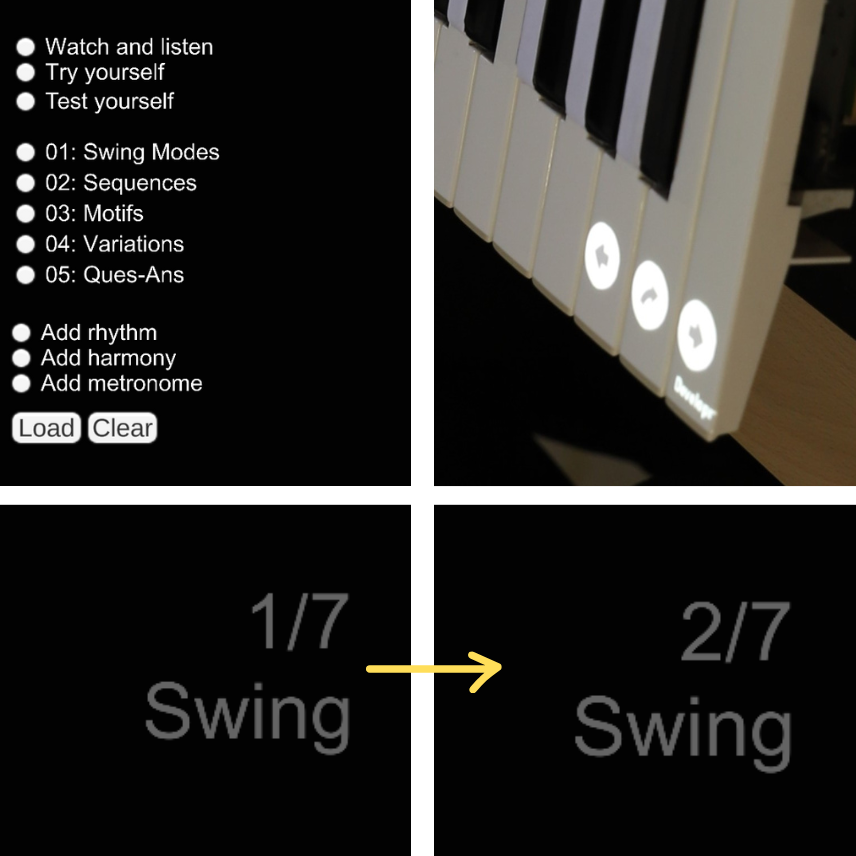
\includegraphics[width=0.45\textwidth]{figs/uicontrol.png}
%   \caption{%
%   	(Top left) ImproVisAR menu which allows the user to select mode first, then a lesson, then an optional guidance or accompaniment. (Top right) Keyboard-based controls on keys A6, B6 and C7. It allows the user to jump back (left), jump next (right) or restart (middle) lesson. (Bottom) Shows the user the current lesson based that the user can navigate with the UI controls. %
%   }
%   \label{fig:menu}
% \end{figure}


\par %The \textit{ImproVisAR} system comes with four modes that learners can choose from (see \autoref{fig:modes}). These are (1) \texttt{Watch-And-Listen}, (2) \texttt{Try Yourself}, (3) \texttt{Test Yourself} and (4) \texttt{Compose-on-the-Fly}. These modes differ in the delivery of the selected lesson to the learner. The \texttt{Watch-And-Listen} mode provides learners with both visualisations and audio feedback. In this mode, the learners are expected to, as the name implies, simply watch and listen on how the lesson is done. This gives the learners a chance to watch (and listen) on how the keys are pressed (by the lighting of the keys and the playing of the \texttt{MIDIout} presses that they hear). This builds on top of the Listen mode done in prior works since the learners are provided with both visual and audio content for them to learn the specific lesson. As the lesson is played, they see the music sheet on top, the animation of the rolling piano bars and the sound of each key press as it hits the keys. 
The \textit{ImproVisAR} system offers four learning modes for users to choose from (see \autoref{fig:modes}): (1) \texttt{Watch-And-Listen}, (2) \texttt{Try Yourself}, (3) \texttt{Test Yourself}, and (4) \texttt{Compose-on-the-Fly}. Each mode delivers the selected lesson to the learner in a different way. In the \texttt{Watch-And-Listen} mode, learners are provided with both visualisations and audio feedback. As the name suggests, learners simply watch and listen to how the lesson is performed. This allows them to observe the key presses (with keys lighting up) and hear the corresponding \texttt{MIDIout} sounds. This mode builds on the Listen approach from previous studies, as it presents both visual and auditory content for learners to understand the lesson. While the lesson is played, users can see the music sheet at the top, the animated piano roll bars, and the sound of each key press as it strikes the keys. They can as well play along.
%The \texttt{Try Yourself} mode provides learners with visualisations alone and does not provide audio feedback. The same content in \texttt{Watch-And-Listen} is provided however, in this mode, it is expected that the learners, ``see to themselves'' the lesson they watched and try it by actually pressing the keys at the right time. The \texttt{MIDIout} events are not played, so when the falling piano bars hit the keys, no sound is produced unless the learner presses them themselves. This is especially obvious when the learner miss to press the keys are they fall. Through this process, the learner are able to see the content and hear the output from their key press alone. With the help of the animations and the timing, the learners are able to see if they are on-time with their presses as the falling piano roll bars go down along the space. 
The \texttt{Try Yourself} mode offers learners visualisations only, without automatic audio feedback. It presents the same content as the \texttt{Watch-And-Listen} mode, but here, learners are expected to actively ``try'' the lesson by pressing the keys at the correct moments. The \texttt{MIDIout} events are not triggered, so no sound is produced when the falling piano bars reach the keys unless the learner presses them. This becomes particularly noticeable if the learner misses a key press. %In this mode, learners can see the visual content and hear only the sound they produce by pressing the keys. The falling bar animations and timing cues help learners gauge if their key presses are on time.

\par The \texttt{Test Yourself} mode does not provide any visualisation or audio feedback to the learner. %Since we are in the context of piano improvisation where they can compose on the fly, the falling piano roll bars are not seen and their respective \texttt{MIDIout} events are not heard as well. During this mode, the learners are given the freedom to simply copy, then play the music sheet notation that they see on top of the interface or compose half-way (either before or after) the 4 bars that are displayed. Across all modes, the metronome is a default provided guidance for the learners. By following a prescribed sequence of \texttt{Watch-And-Listen}, then \texttt{Try Yourself} and lastly \texttt{Test Yourself}, the learners go through the Listen-Imitate-Try approach and undergo the Attention-Retention-Reproduction phases of SLT. Learners select a mode first and then select a lesson that they wish to learn. Anytime in between these modes they can turn on or off any additional guidance that they may need most especially depending on the current lesson they are learning.
This mode focuses on allowing learners to compose on the fly. The falling piano roll bars and corresponding \texttt{MIDIout} events are thus absent. In this mode, learners have the freedom to either replicate the music sheet notation displayed at the top of the interface or compose halfway through the 4-bar section. The metronome remains available as a default guide across all modes. Learners typically follow a sequence—starting with \texttt{Watch-And-Listen}, progressing to \texttt{Try Yourself}, and concluding with \texttt{Test Yourself}--which aligns with the Listen-Imitate-Try approach and the Attention-Retention-Reproduction stages of Social Learning Theory (SLT). %Learners can select a mode and lesson to work on, and can toggle additional guidance on or off depending on their needs for each lesson.

\par %\textit{ImproVisAR} has the \texttt{Compose-on-the-Fly} mode where the learner of the system is given an opportunity to improvise and take turns with the system. In this mode, \textit{ImproVisAR} provides the learner with the first half of the melody (both in improvisation and music sheets), played ala \texttt{Watch-and-Listen} mode, and then the second half of the bars provide gaps for the learner to play. During this second half, harmony audio is played, harmony keys are lit but there are no falling piano bars or no notes in the music sheet displayed which we hope should give the learner the freedom and boost it needs to compose on the fly. This mode is only available for Lessons 04 and Lesson 05. The sequence is visualised as seen in \autoref{fig:ques-ans}.  
The last mode featured is \texttt{Compose-on-the-Fly} mode, which offers learners the chance to improvise and alternate turns with the system. In this mode, the system plays the first half of the melody (both as an improvisation and with accompanying music sheets) in a similar way to the \texttt{Watch-and-Listen} mode. For the second half, gaps are provided for the learner to play. During this phase, harmony audio plays, and harmony keys are illuminated, but there are no falling piano bars or displayed notes on the music sheet. This design is intended to give the learner the freedom and confidence to improvise. This mode is only available for Lessons 04 and 05 and is visualised in the sequence shown in \autoref{fig:ques-ans}.

% \subsubsection{Watch-And-Listen}
% \subsubsection{Try Yourself}
% \subsubsection{Test Yourself}

\subsection{Lessons}
\label{subsec: lessons}

\par %Part of the our main contribution is the organisation of the different lessons in our \textit{ImproVisAR} system, most especially on how they work best with the different learning modes (which we have described in \autoref{subsec: modes}) and the various guidance support we have described earlier (in \autoref{subsec: design}). While we understand that improvisation as well comes in various forms and genre, we have decided to narrow our focus on jazz improvisation with the piano. Our Lessons were developed, curated and organised with the help of our collaborators who are experts in teaching jazz and piano improvisation. We designed five (5) lessons, the contents are built on top of each other which the expectation, that if followed by the learner user, ultimately leads to the main task of being able to compose on the fly. These lessons are also the core elements that are present in the \texttt{sibelius file}. These lessons were derived from a co-design process that identified different learning objectives (by teachers) and then mapped to their equivalent applicable tools (for developers)~\cite{deja2024teach}. The complete list of lessons are seen in the interface, that the user can choose from. Most lessons are also broken down in sublessons which are usually composed of 8 sub lessons (except for Swing which has 7 sub parts).
A key aspect of our contribution lies in how we organise the lessons within the \textit{ImproVisAR} system, particularly in aligning them with the different learning modes (discussed in \autoref{subsec: modes}) and the various guidance supports (outlined in \autoref{subsec: design}). Recognising that improvisation spans various forms and genres, we chose to focus specifically on jazz piano improvisation. As mentioned, the lessons were developed, curated, and structured with the assistance of experts in jazz and classical piano improvisation teaching. Through a co-design process, the experts identified learning objectives that developers mapped to relevant tools~\cite{deja2024teach}.
We designed five lessons that build progressively on one another, with the goal of guiding learners towards the ultimate skill of composing on the fly. These lessons form the core content within the \texttt{sibelius file}. Users can select from the complete list of lessons in the interface, with most lessons broken into eight sub-lessons (except for the Swing lesson, which has seven parts).
%These are seen and can be controlled by jumping to the next or jumping back to the next sub lesson (see \autoref{fig:menu} Bottom left and Bottom right). 
%We describe this mapping and each lesson in greater detail below. %A preview of the music sheets for each lesson are seen in \autoref{appendix:lesson} \autoref{fig:all_lessons}. 

\par %\textbf{Lesson 01: Swing.} Our experts recommend that learners begin with being familiar with learning the different modes and extensions at first. To make things easier, we did this by focusing on the different modes starting from the C-key. The tools needed here involved showing the different modes (e.g. \texttt{Ionian} which starts in \texttt{C} as subtask 1 out of 7, \texttt{Dorian} which starts in \texttt{D} displayed as subtask 2 out of 7 and so on, until \texttt{Locrian} which starts in \texttt{B} displayed as Lesson 7 out of 7 in the interface). Thus, Lesson 01 Swing shows all modes and  how to play them in swing, in 4 bars each and with at least another repetition. By being able to \texttt{Watch-and-Listen}, they get to watch each lesson at most 4 times. 
\textbf{Lesson 01: Swing.} The experts recommend that learners start by becoming familiar with the different modes and their extensions. To simplify this, we focus on the modes beginning with the C-key. The tools used here involve showing each mode (e.g. \texttt{Ionian} starting on \texttt{C} as subtask 1 of 7, \texttt{Dorian} starting on \texttt{D} as sub-task 2 of 7, and so on, up to \texttt{Locrian} starting on \texttt{B}, which is displayed as Lesson 7 of 7 in the interface). Thus, \texttt{Lesson 01: Swing} introduces all the modes and demonstrates how to play them in swing rhythm, with 4 bars each and at least one repetition. Using the \texttt{Watch-and-Listen} mode, learners can watch each mode up to four times.

\par %\textbf{Lesson 02: Sequences.} After learning and getting to play across different modes in swing, understanding motifs through different sequences of notes that sound great together is the next step. This is done by being able to repeat motif sequences and learn how to rearrange them. This time, we focused on forming new motifs across the \texttt{Dorian} scale which starts in \texttt{D} because we are following the \texttt{ii-V-i} harmonic progression which begins with the \texttt{Dm7} chord. They are introduced to different sequences that go from \texttt{Up-up}, \texttt{Up-Down}, \texttt{Down-Down}, \texttt{Down-Up} along with their respective extensions (a total of 8 sub-lessons in total). The sub-tasks cover 4 bars and by following a \texttt{Watch-and-Listen} mode, they get to each each lesson  twice. 
\textbf{Lesson 02: Sequences.} After mastering the different modes in swing, the next focus is on understanding motifs through various sequences of notes that harmonise well together. This involves repeating and rearranging motif sequences. In this lesson, we concentrate on creating new motifs within the \texttt{Dorian} scale, starting on \texttt{D}, and following the \texttt{ii-V-i} harmonic progression that begins with the \texttt{Dm7} chord. Learners are introduced to various sequences such as \texttt{Up-Up}, \texttt{Up-Down}, \texttt{Down-Down}, and \texttt{Down-Up}, along with their extensions, comprising a total of 8 sub-lessons. Each sub-task spans 4 bars, and learners can review each lesson twice using the \texttt{Watch-and-Listen} mode.

\par %\textbf{Lesson 03: Motifs.} The goal of this lesson is now to be familiar with different rhythmic patterns which are the core of motifs themselves. Our experts believe that we can do this by allowing them to practice by repeating motifs and then being able to invent their own motifs as well. Following the same harmonic progression in the \texttt{Dorian} scale, the learners are introduced to different motifs as rhythmic patterns that they can practice and play with. Similar to Lesson 02, the lessons are shown across 4 bars and can be practised twice. 
\textbf{Lesson 03: Motifs.} In this lesson, the focus shifts to becoming familiar with various rhythmic patterns, which are fundamental to creating motifs. Our experts suggest that learners should practice repeating existing motifs and then create their own. Sticking with the \texttt{Dorian} scale and its harmonic progression, this lesson presents different rhythmic patterns that learners can practice and experiment with. As with Lesson 02, each motif is displayed across 4 bars, and learners have the opportunity to practice each one twice.

\par %\textbf{Lesson 04: Variations.} By being familiar with the different motifs (and the rhythmic patterns that come from them), the students should be able to learn and practice phrasing, which are longer than motifs. This lesson was designed with the same \texttt{ii-V-i} and \texttt{ii-V-i-VI} progression where they are also introduced to different chord tones. They are also introduced with a core melody and are taught how to play them differently while still being able to retain the same melody in their phrases. They also get to repeat phrases over different chords in the said progression. Our collaborators believe that through this lesson, they are able to recognise the relationship between melody and harmony which equips them with tools on how to complete their would-be compositions. 
\textbf{Lesson 04: Variations.} Building on their understanding of motifs and rhythmic patterns, students are now introduced to phrasing, which involves creating longer musical passages. This lesson continues with the \texttt{ii-V-i} and \texttt{ii-V-i-VI} progressions and introduces different chord tones. Students are given a core melody and learn how to vary it while maintaining the same melodic structure in their phrases. They practice repeating these phrases over various chords within the progression. According to experts, this lesson helps students grasp the relationship between melody and harmony, providing them with essential skills for developing their compositions.

\par %\textbf{Lesson 05: Question and Answer.} Lastly, this lesson acts as a summative exercise where they apply basic composition techniques through an approach of the similar name. This lesson is presented differently across the different modes. In \texttt{Watch-and-Listen}, students are presented with visualisations that allow them to repeat questions (first two bars out of four) and repeat answers (second two bars out of four). This creates some sort of a dialogue where an initial melody is provided and students are shown at least four different ways to answer this given melody. In \texttt{Try Yourself}, they are presented with the same set as that of \texttt{Watch-and-Listen}, and get to try out the four different ways of ``answering'' the given melody. The \texttt{Test Yourself} mode is most interesting as they are given the same set of ``question'' melody but this time they are now expected to give their own ``answer'', coming from the experience of trying out the four previous ``answers'' they just recently-tried. Visualisations (in form of sheets or falling bars) for any answer are not shown in this specific mode. With prior knowledge of the modes and the familiarity of the vocabulary they learned from motifs and sequences, they are expected to improvise and compose on the fly. They should be able to apply different styles and apply rhythmic patterns from the previous lessons they have seen in the system. The learners are expected to practice and compose their own melody or play a recent one they heard to the given melody question. 
\textbf{Lesson 05: Question and Answer.} This final lesson serves as a comprehensive exercise where students apply basic composition techniques using a ``question and answer'' approach. The lesson varies across the different modes. In \texttt{Watch-and-Listen}, students view visualisations that allow them to repeat questions (the first two bars of a four-bar phrase) and answers (the last two bars). This setup simulates a musical dialogue where students see at least four different ways to respond to a given melody. In \texttt{Try Yourself}, students are given the same content as in \texttt{Watch-and-Listen} and have the opportunity to experiment with the four different ways to respond to the melody. The \texttt{Test Yourself} mode is particularly engaging as students receive the same ``question'' melody but are expected to create their own ``answer'', drawing from their experience with the four previously tried responses. In this mode, no visualisations (whether in the form of sheet music or falling bars) are provided. Students are expected to use their knowledge of the modes and the vocabulary learned from motifs and sequences to improvise and compose on the fly. They should be able to incorporate various styles and rhythmic patterns from previous lessons to either create a new melody or perform a recent one they have learned in response to the given melody question.

\subsection{Technical Aspects}

\par %We combine all these features into an interactive space with overlaid projections, lit keys and surround sound system inspired by the works of~\cite{rogers2014piano, weing2013piano}. We connected an overhead \texttt{Barca} projector, a modified \texttt{Kurzweil v2003} Clavinova with raised keys and a laptop computer in an interactive space (see \autoref{fig:teaser} Middle). The clavinova was connected with through a Yamaha USB music interface on a Macbook Pro and with \texttt{Garageband}. The \textit{ImproVisAR} system was developed over \texttt{Unity} which communicated with the clavinova through the \texttt{RtMidi API}\footnote{\url{https://github.com/matthewcpp/ABCUnity}} which detected the keypress events across the system. The setup was connected to a 360 sound system with a standard bass sub-woofer and a receiver that connected multiple satellite speakers to ensure an immersive sound experience. An ergonomic seat along that can be rotated is included in the setup where users can easily-adjust the height to their own comfort. 
% midi protocol to detect presses. information. notes. midi. playback 
We integrate the features described above into an interactive setup that includes overlaid projections, illuminated keys, and a surround sound system, drawing inspiration from the works of~\cite{rogers2014piano, weing2013piano}. The setup consists of an overhead \texttt{Barca} projector, a modified \texttt{Kurzweil v2003} clavinova with raised keys, and a laptop computer (see \autoref{fig:teaser} Middle). The clavinova is connected to a MacBook Pro via a Yamaha USB music interface and \texttt{Garageband}. The \textit{ImproVisAR} system is developed in \texttt{Unity} and communicates with the clavinova through the \texttt{RtMidi API}\footnote{\url{https://github.com/matthewcpp/ABCUnity}}, which tracks keypress events across the system. This setup is linked to a 360-degree sound system, featuring a standard bass subwoofer and a receiver that connects multiple satellite speakers to create an immersive audio experience. Additionally, the setup includes an ergonomic, height-adjustable rotating seat for user comfort.

\section{Pilot Study Evaluation}

\par %We wanted to evaluate initially \textit{ImproVisAR} in terms of usability and user experience. We conducted a within-subject study that involved two tasks namely Task 1: Jazz in Swing Mode and Task 2: Compose-on-the-Fly. We wanted to do this in-comparison to the traditional approach of using music sheets (similar to that of the protocol in the works of ~\cite{rogers2014piano}). Specifically, we wanted to compare the effects of the piano roll visualisation versus the traditional way of learning the piano with sheet music. On both tasks we recruited six ($n=6$) participants who had prior knowledge on the piano (avg. 8.33 years of exp, avg age 21, 5M, 1F), can confidently-read piano sheets and are computer literate). All participants were able to perform both tasks on both systems in a counter-balanced order. We wanted to measure their subject cognitive load~\cite{hart1988development} and subjective user experience~\cite{schrepp2017design} after doing each task on both conditions. 
The aim of the pilot study was to assess the usability and user experience of \textit{ImproVisAR} through an initial evaluation. We conducted a within-subject study with two tasks: Task 1—Jazz in Swing Mode, and Task 2—Compose-on-the-Fly. This evaluation compared the \textit{ImproVisAR} system to the traditional method of using sheet music only, similar to the protocols outlined in~\cite{rogers2014piano}. Specifically, we sought to compare the effectiveness of piano roll visualisations against conventional music sheet learning for complex music concepts with advanced students. For this study, we recruited six participants ($n=6$) with prior piano experience (average of 8.33 years, average age 21, 5 males and 1 female), who were proficient in reading music sheets . Each participant completed both tasks using both systems in a counter-balanced order. We measured their cognitive load~\cite{hart1988development} and subjective user experience~\cite{schrepp2017design} after performing each task under both conditions.

% \begin{figure*}[tbp]
%   \centering
%   \begin{subfigure}[b]{0.27\textwidth}
%   	\centering
%   	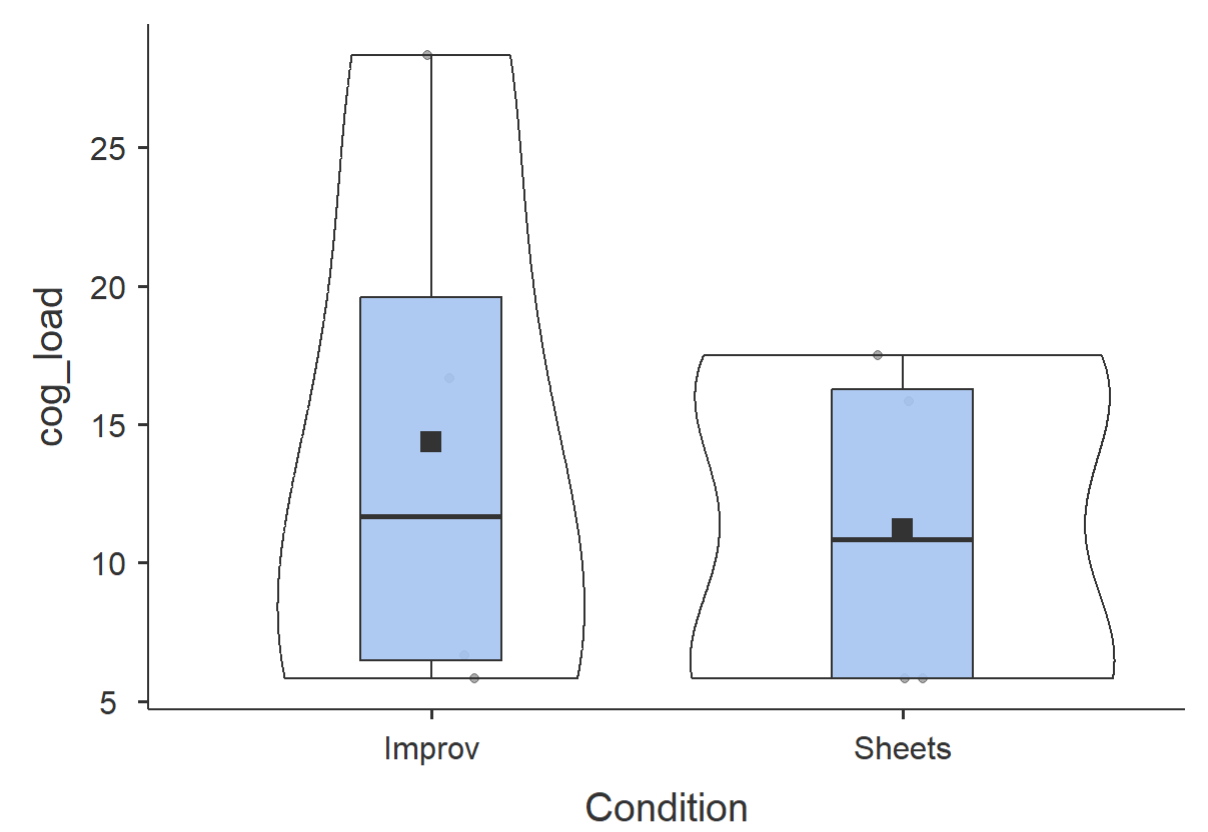
\includegraphics[width=\textwidth]{figs/cogload_1.png}
%   	\caption{Cognitive load for Task 1}
%   	\label{fig:cogload_task1}
%   \end{subfigure}%
%   \begin{subfigure}[b]{0.27\textwidth}
%   	\centering
%   	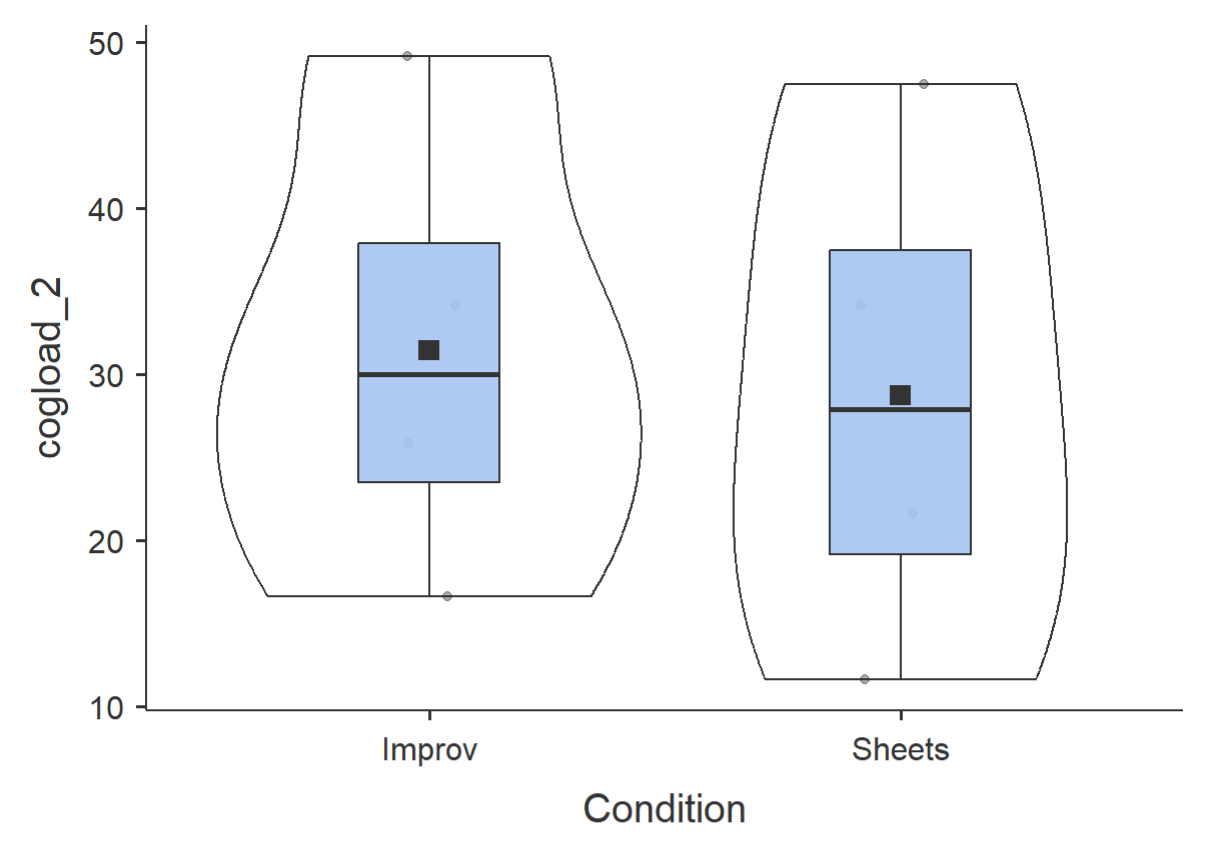
\includegraphics[width=\textwidth]{figs/cogload_2.png}
%   	\caption{Cognitive load for Task 1}
%   	\label{fig:cogload_task2}
%   \end{subfigure}%
%   \begin{subfigure}[b]{0.27\textwidth}
%   	\centering
%   	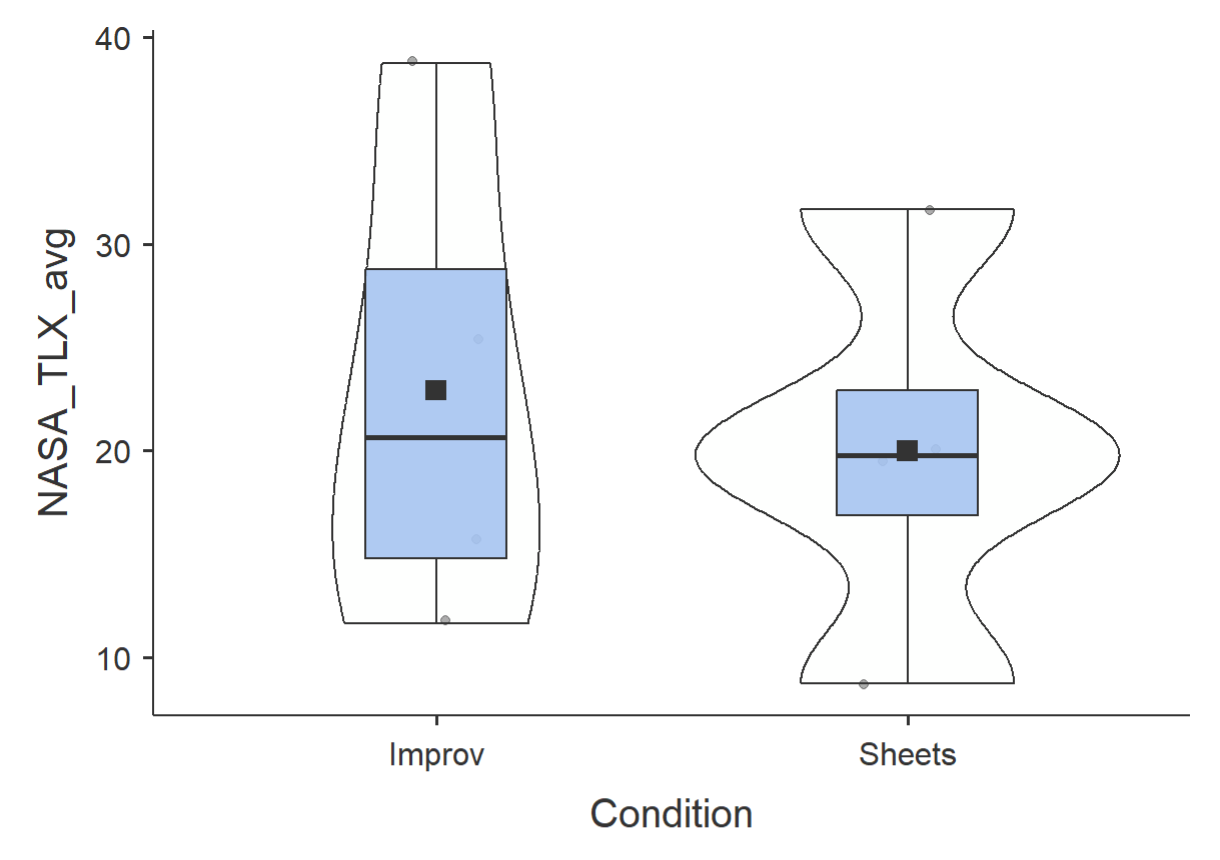
\includegraphics[width=\textwidth]{figs/cogload_avg.PNG}
%   	\caption{Average Cognitive Load across Two Tasks}
%   	\label{fig:avg_coglaod}
%   \end{subfigure}%
%   \\%
%    \begin{subfigure}[b]{0.27\textwidth}
%   	\centering
%   	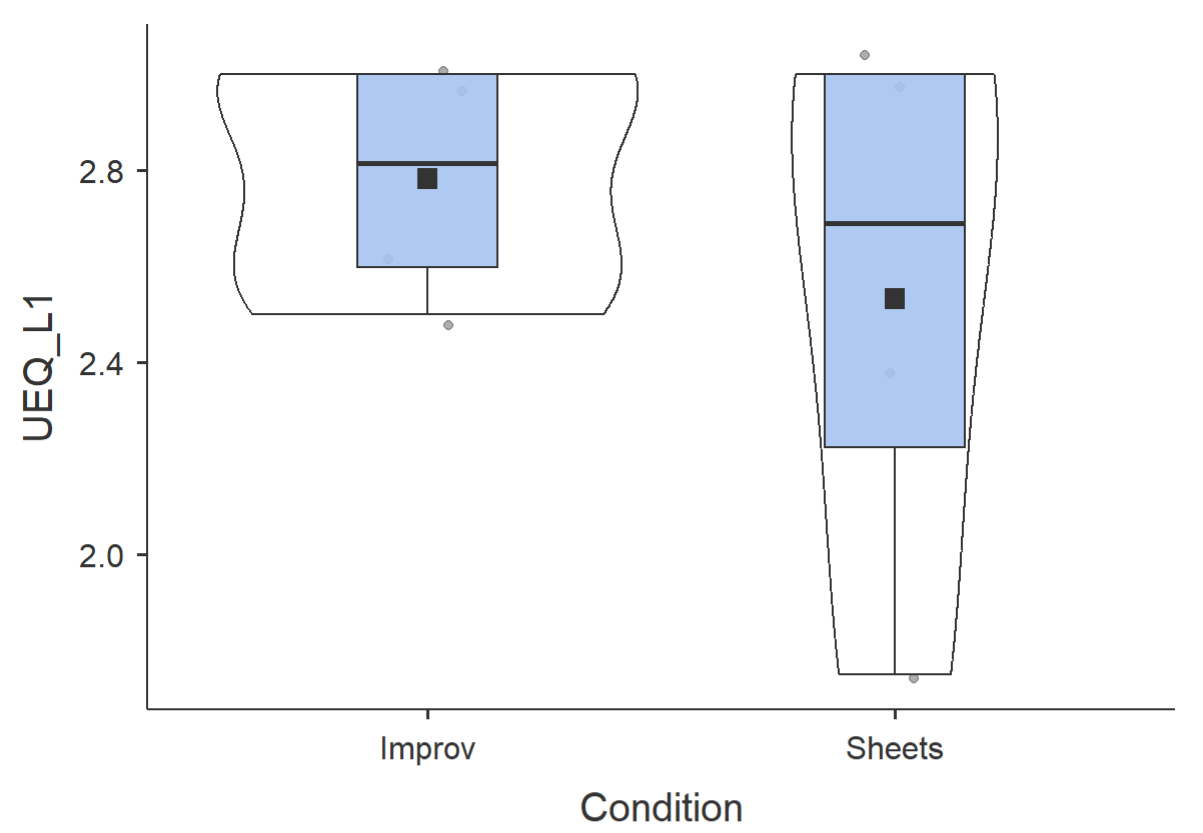
\includegraphics[width=\textwidth]{figs/ueq_t1.PNG}
%   	\caption{UEQ for Task 1}
%   	\label{fig:ueq_task1}
%   \end{subfigure}%
%     \begin{subfigure}[b]{0.27\textwidth}
%   	\centering
%   	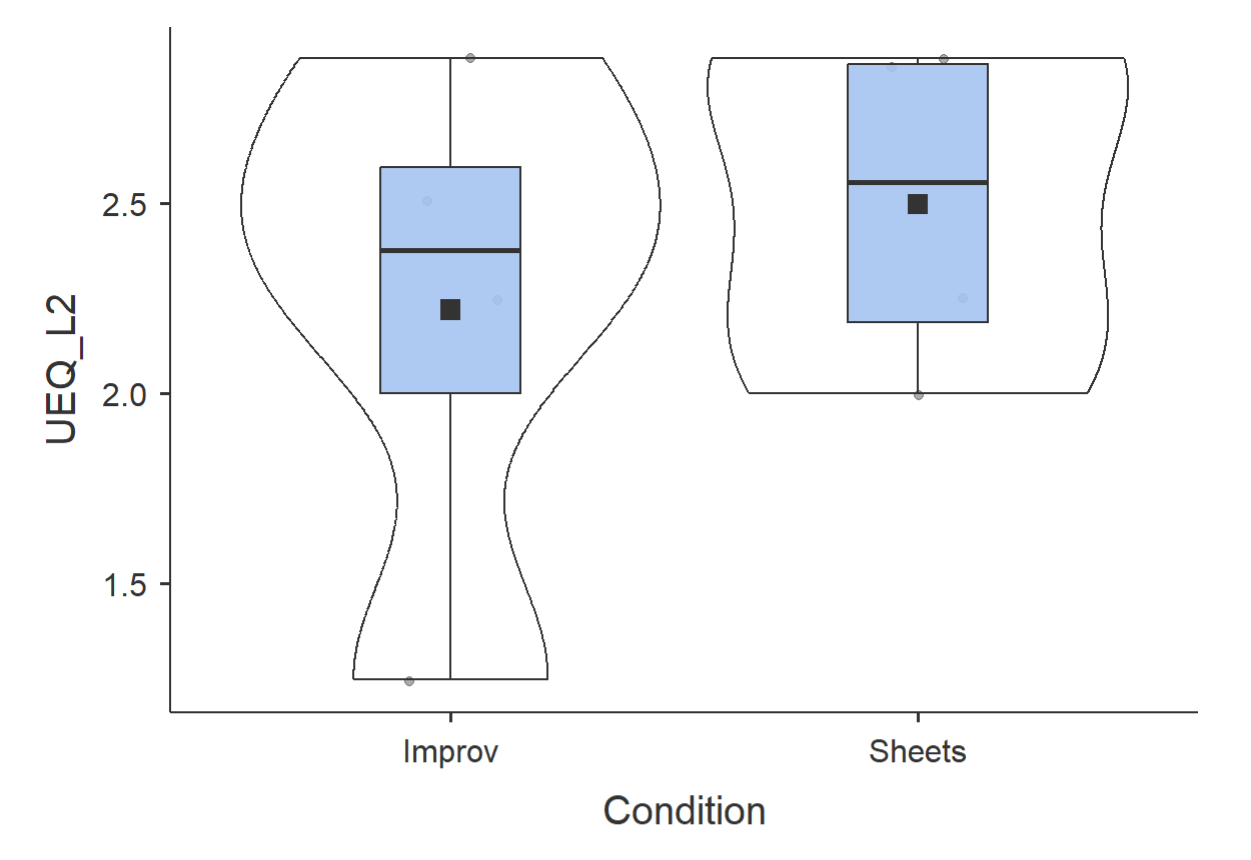
\includegraphics[width=\textwidth]{figs/ueq_t2.PNG}
%   	\caption{UEQ for Task 2}
%   	\label{fig:ueq_task2}
%   \end{subfigure}%
%     \begin{subfigure}[b]{0.27\textwidth}
%   	\centering
%   	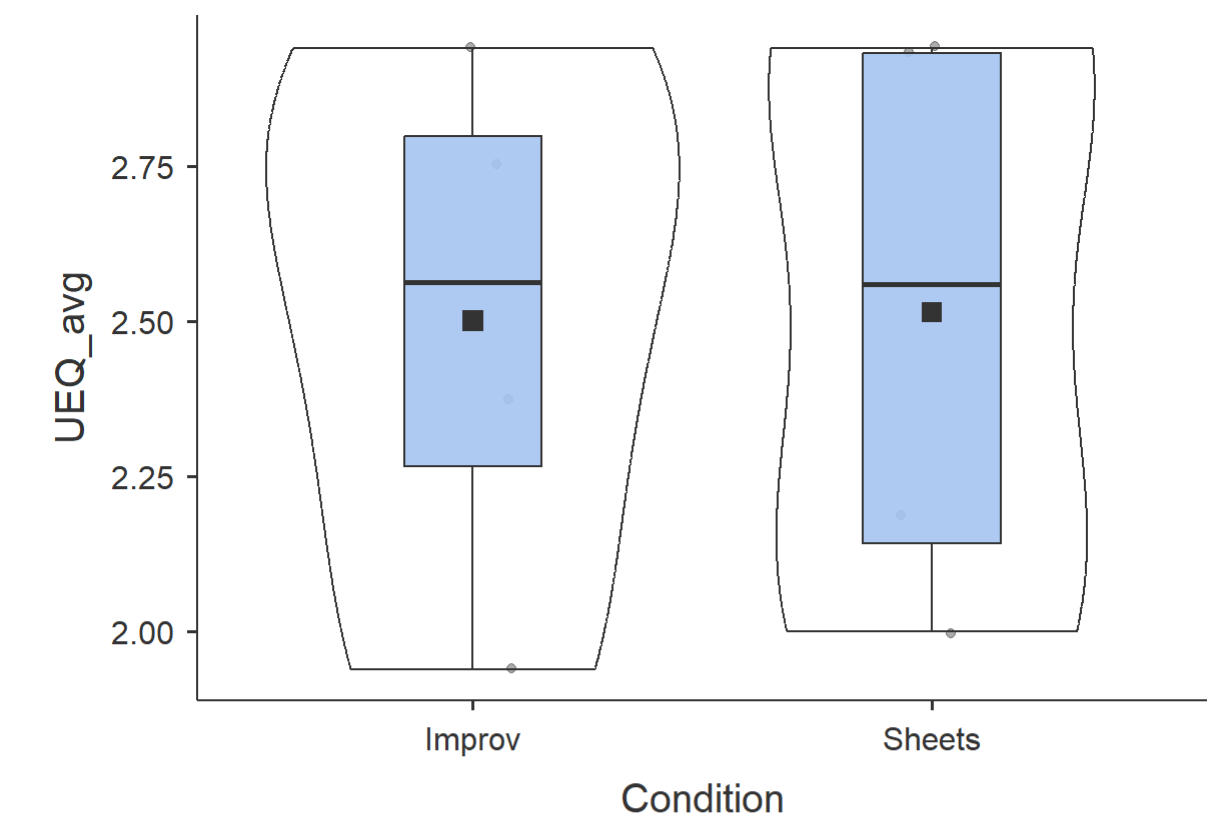
\includegraphics[width=\textwidth]{figs/ueq_2cond.PNG}
%   	\caption{Average UEQ across two Tasks}
%   	\label{fig:avg_ueq}
%   \end{subfigure}%
%   \\%
%     \begin{subfigure}[b]{0.75\textwidth}
%   	\centering
%   	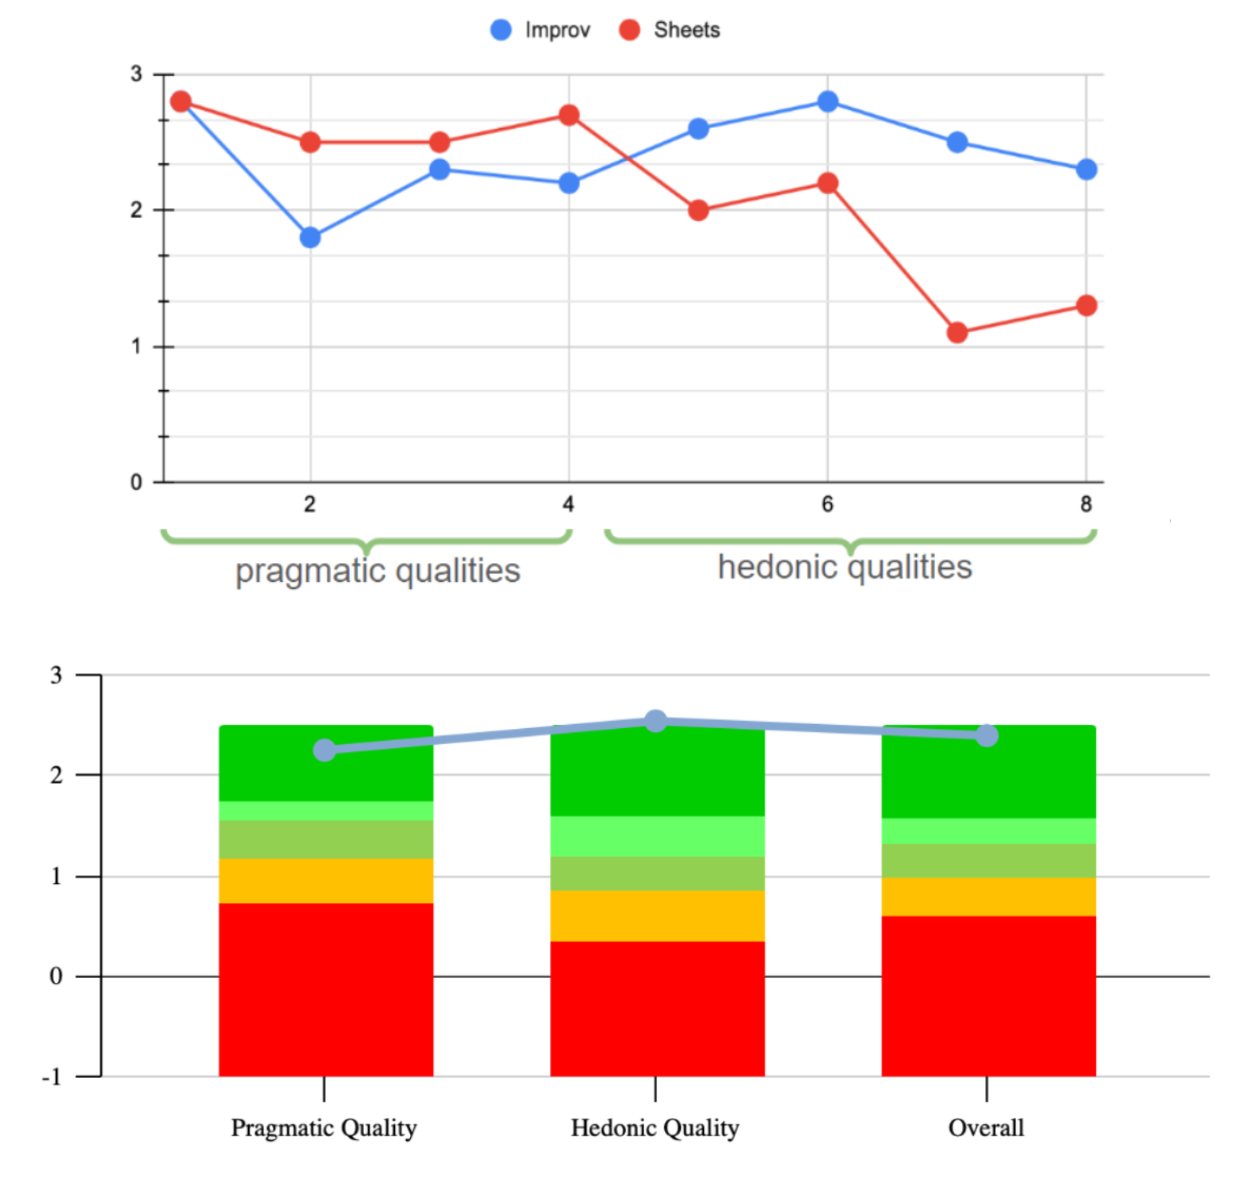
\includegraphics[width=\textwidth]{figs/ueq_overall.png}
%   	\caption{(Left) Comparison of UEQ means between ImproVisAR and Sheets. \hspace{4cm} (Right) UEQ Rating based on Industry Benchmark.}
%   	\label{fig:ueq_overall}
%   \end{subfigure}%
%   \subfigsCaption{Various figures showing different plots of cognitive load and UEQS rating collected during our pilot evaluation.}
%   \label{fig:ex_subfigs}
% \end{figure*}

% \begin{figure}[tb]% specify a combination of t, b, p, or h for top, bottom, on its own page, or here
%   \centering % avoid the use of \begin{center}...\end{center} and use \centering instead (more compact)
%   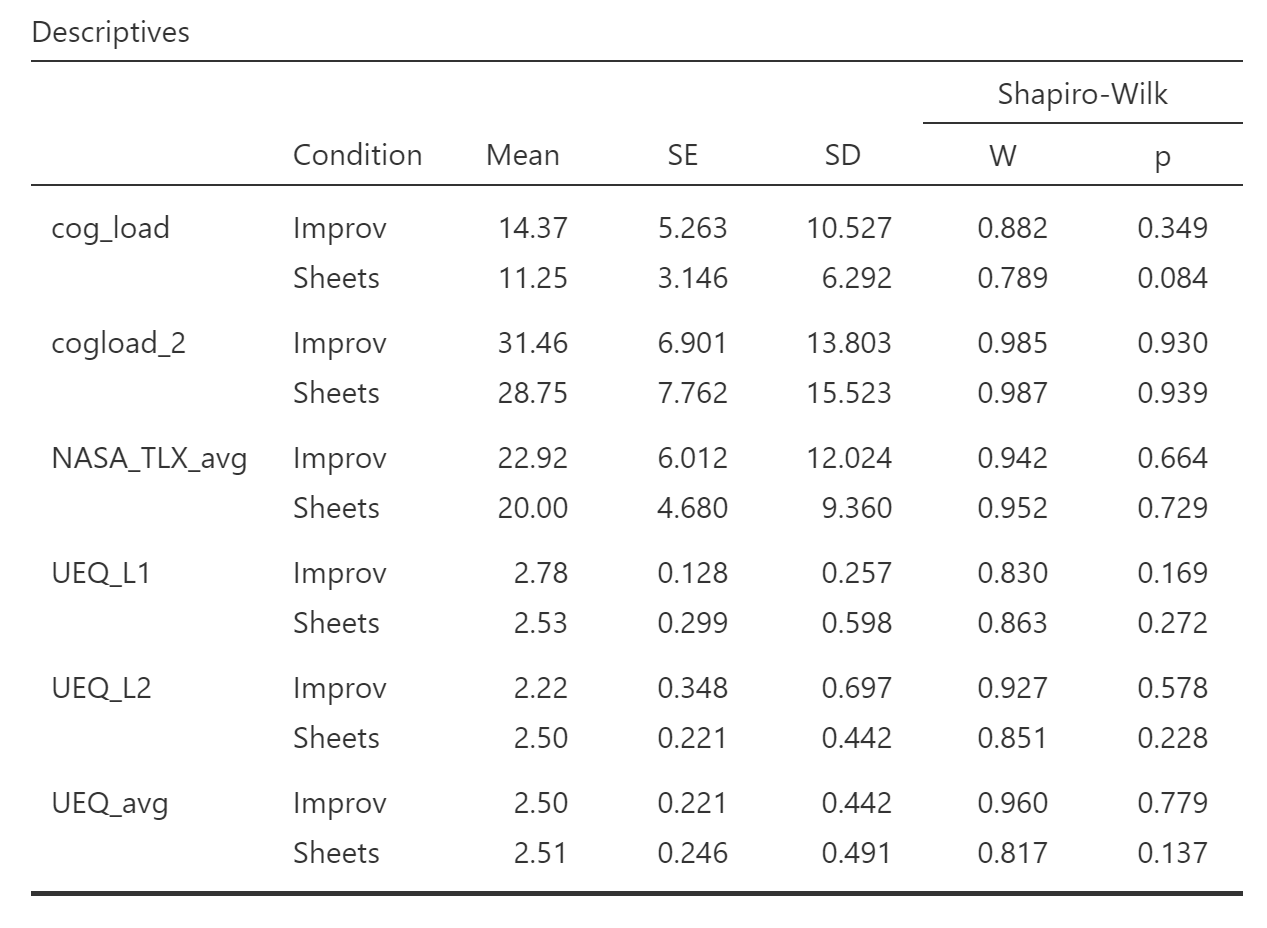
\includegraphics[width=\columnwidth]{figs/descriptives.PNG}
%   \caption{%
%   	descriptive statistics%
%   }
%   \label{fig:descriptive-statistics}
% \end{figure}


\subsection{Experiment Setup}
\par The \textit{ImproVisAR} space was  configured as illustrated in \autoref{fig:teaser}. For the Sheets condition, we used the same setup and projected the music sheets onto the surface at the same angle and position as the piano roll visualisation in the \textit{ImproVisAR} system. The sound settings were consistent for both conditions, with audio output provided by a surround sound system connected to the computer. In both conditions, we used Garageband, a well-known digital audio workstation for musicians, to record key presses and performances. This approach ensured consistent quantitative  measurements of performance, allowing us to record they different key press events and their corresponding pitch sounds. 

\subsection{Task 1: Learn Modes using Swing}
In a within-subject study comparing the two conditions, we evaluated the subjective cognitive load and user experience of participants as they learned different modes in Swing and practiced them using only their right hand. We hypothesised that learning modes in Swing with \textit{ImproVisAR} would result in a lower subjective cognitive load compared to tradition music sheet reading. Similarly, we anticipated that the user experience with \textit{ImproVisAR} would be rated more favorably than the traditional approach. 

\par At the beginning of the session, participants filled out a questionnaire about their demographic information, musical background, and provided their informed consent. Each participant interacted with both systems and learned the same lesson with each system. The order in which they used the systems was counterbalanced to avoid biases related to novelty and familiarity. After learning and playing the lesson with each system, participants completed a 6-item NASA TLX questionnaire~\cite{hart1988development}, followed by the short version of the UEQ questionnaire~\cite{schrepp2017design}. The task lasted approximately 10 minutes. 

\subsection{Task 2: Compose On The Fly}

\begin{figure}[tb]% specify a combination of t, b, p, or h for top, bottom, on its own page, or here
  \centering % avoid the use of \begin{center}...\end{center} and use \centering instead (more compact)
  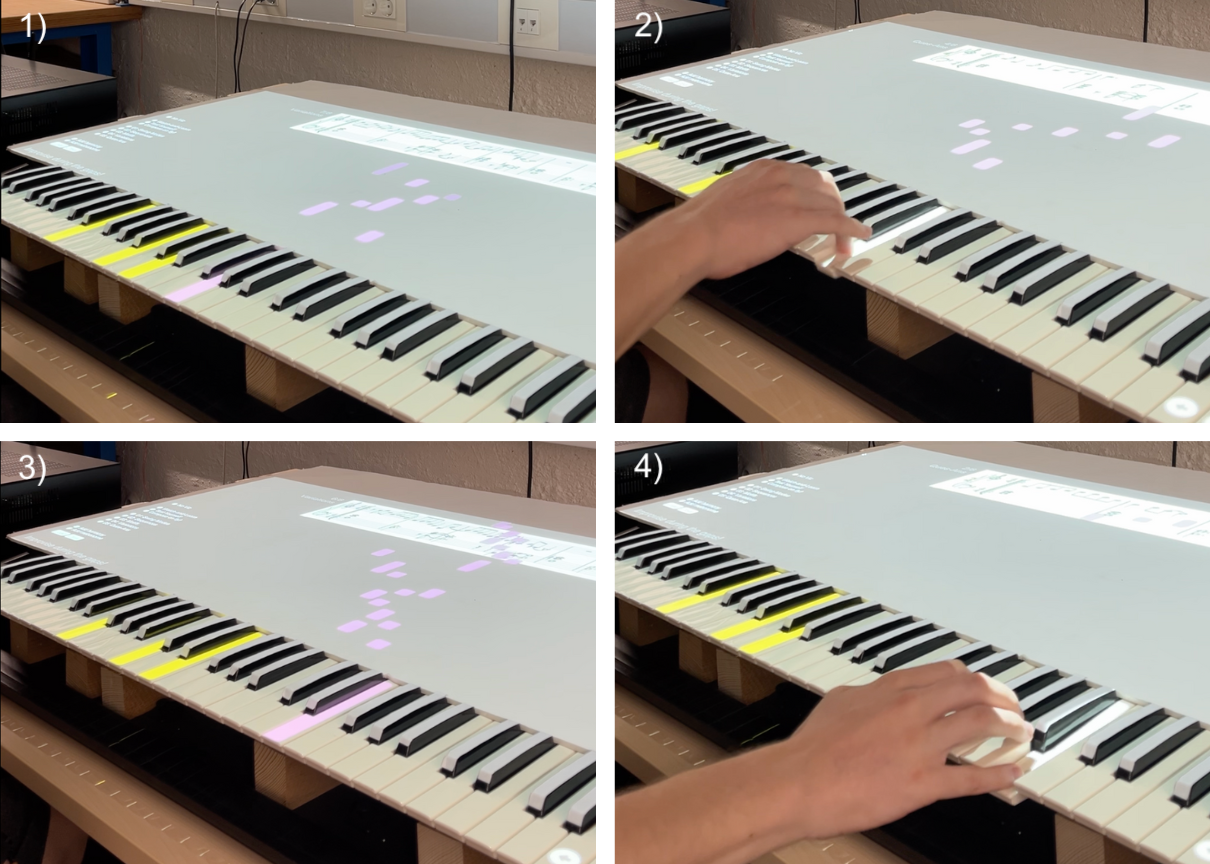
\includegraphics[width=\columnwidth]{figs/ques-ans.png}
  \caption{%
    Lesson 05: Question and Answer in \texttt{Compose-on-the-Fly} mode. In \textbf{1)} the learner is presented with both melody and harmony along with their visualisations and audio playback (approximately 2 measure bars). In the music sheets, the respective notes are also displayed (refer to \autoref{fig:modes} Right). Learners play during the gap of 2 measure bars in \textbf{2)}. Harmony audio continues to play and keys remain illuminated, helping them maintain the current scale. This process is repeated, and in \textbf{3)}, the learner observes the same setup. When the gap appears again, they are encouraged to play and improvise on their own as shown in \textbf{4)}.
  }
  \label{fig:ques-ans}
\end{figure}

\par We followed the same protocol (\texttt{Watch-And-Listen}, then \texttt{Try Yourself} and then \texttt{Test Yourself}) for this task. But instead of using Lesson 01, we used Lesson 04: Variations. This time, the same group of participants were given the option of either (a) replicating the lesson they learned or (b) composing on the fly based on the melody they just learned. We also measured subjective cognitive load and user experience after each task in each system. For this task, participants had a practice trial and an actual trial (we refer as Trial 1 and Trial 2 respectively) where their performances were recorded and were evaluated by our experts. This task lasted approximately 10 minutes as well.

\subsection{Preferences between two systems}

\par After performing both tasks and collecting ratings on subjective cognitive load and user experience, we also aimed to determine  participants'  preferences between the two systems. We used a set of questions based on the instrument employed in~\cite{banquiero2024color}. The questions were: (PF1) Which one did you like the most? \textit{ImproVisAR} or the Sheets?, (PF2) Which one do you think is better for music learning? \textit{ImproVisAR} or the Sheets?, (PF3) Which one was easier for you to handle? \textit{ImproVisAR} or the Sheets?, (PF4) Which one would you recommend to your colleagues? \textit{ImproVisAR}? Sheets? Both? Neither?, (PF5) Would you like your teacher to use them in class? \textit{ImproVisAR}? Sheets? Both? Neither? and (PF6) Open comments. For questions PF1-PF3, the answers were between two systems while for PF4 and PF5 where based on 4 options (\textit{ImproVisAR}, Sheets, Both or Neither). 

\subsection{Findings}

\subsubsection{Cognitive Load and User Experience Rating}
\begin{figure}[tb]% specify a combination of t, b, p, or h for top, bottom, on its own page, or here
  \centering % avoid the use of \begin{center}...\end{center} and use \centering instead (more compact)
  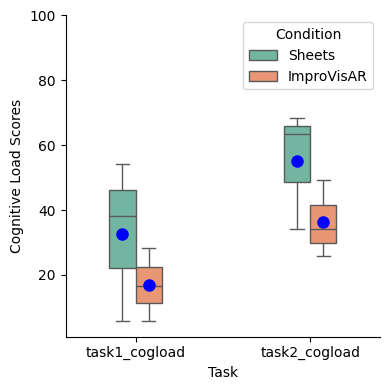
\includegraphics[width=0.5\linewidth]{figs/cog_load_tasks.png}
  \caption{%
  Cognitive Load values of participants during Task 1 and Task 2 for \textit{ImproVisAR} and Sheets condition. %
  }
  \label{fig:cogloadplots}
\end{figure}

\par %We see in \autoref{fig:cogloadplots} a visual summary of all our cognitive load findings from the NASA-TLX questionnaire. We compared the cognitive load values of participants doing Task 1 with Sheets and those doing the same task but with \textit{ImproVisAR}. We also did the same with Task 2. Generally, cognitive load values shows higher trends (more demanding) with Sheets condition compared to when using the \textit{ImproVisAR} system. These findings echo some of the observations found in the study of ~\cite{rogers2014piano, wristen2006demographics} where intrinsic and extrinsic cognitive load were measured to be lower after being exposed to falling piano roll visualisations as opposed to music sheet notations.
In \autoref{fig:cogloadplots}, we present a visual summary of cognitive load findings from the NASA-TLX questionnaire. We compared the cognitive load ratings of participants performing Task 1 using Sheets with those performing the same task using \textit{ImproVisAR}. A similar comparison was made for Task 2. Overall, the cognitive load values were higher (indicating greater demand) for the Sheets condition compared to \textit{ImproVisAR}. These results align with observations from studies such as~\cite{rogers2014piano} and~\cite{wristen2006demographics}, which found that falling piano roll visualisations generally resulted in lower intrinsic and extrinsic cognitive load compared to traditional music sheet notation.

\begin{figure}[tb]% specify a combination of t, b, p, or h for top, bottom, on its own page, or here
  \centering % avoid the use of \begin{center}...\end{center} and use \centering instead (more compact)
  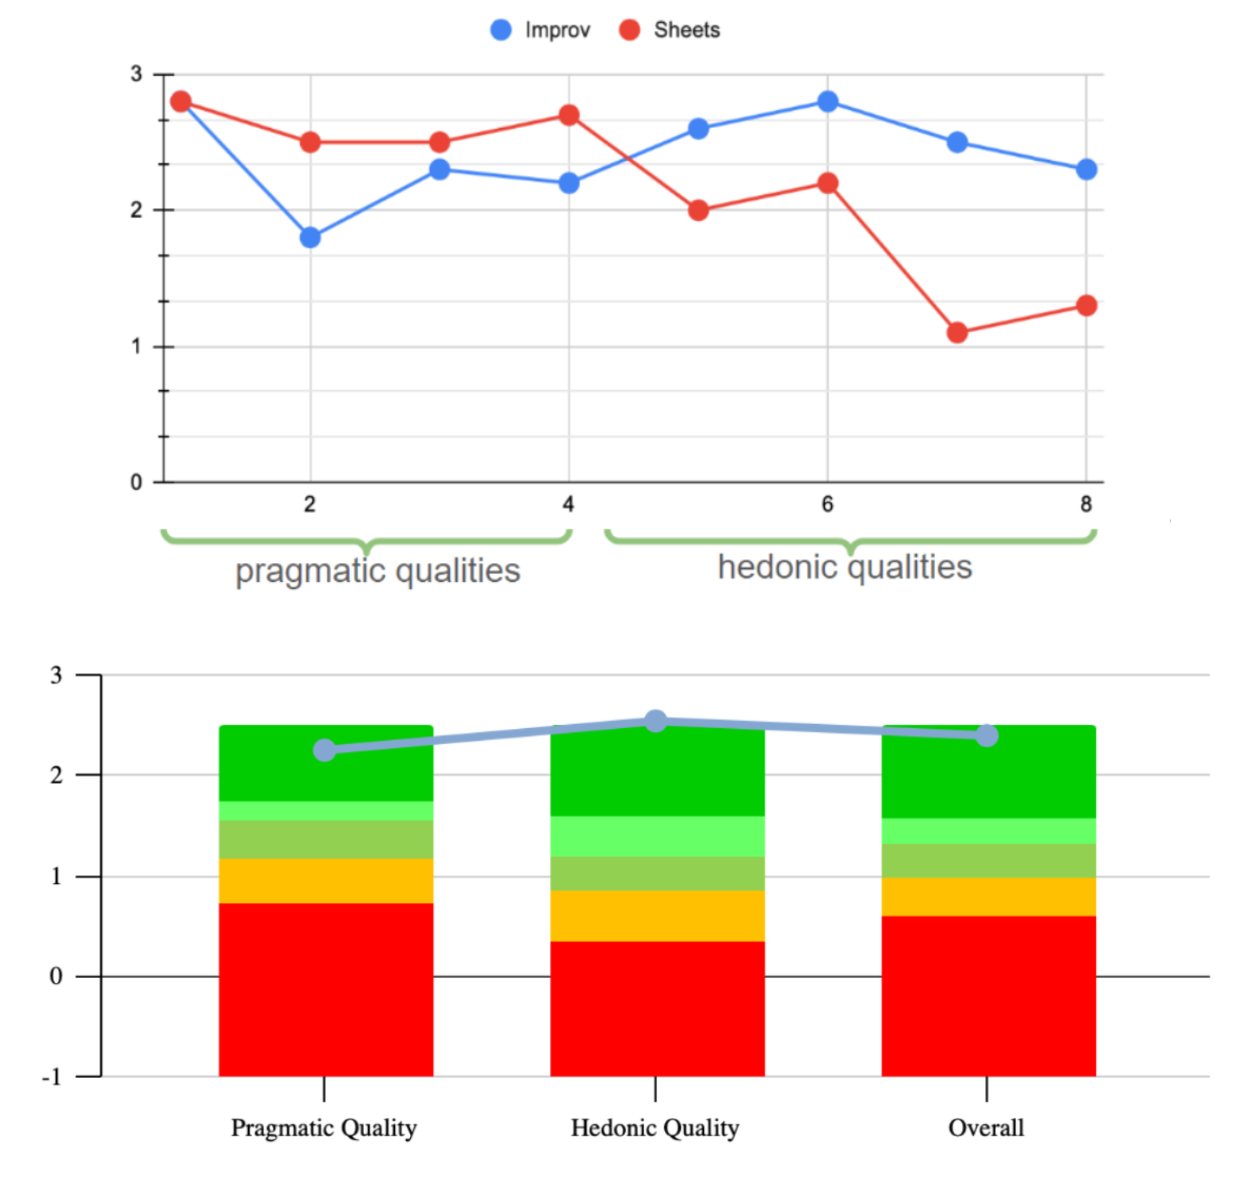
\includegraphics[width=\columnwidth]{figs/ueq_overall.png}
  \caption{%
  User Experience results rated using UEQ-S. \textbf{Top} shows comparison of values between pragmatic and hedonic qualities. \textbf{Bottom} shows UEQ-S of \textit{ImproVisAR} based on UEQ-S ratings. %
  }
  \label{fig:ueqoverall}
\end{figure}

\par %We also show in \autoref{fig:ueqoverall} our user experience results from the UEQS questionnaire. User Experience rating for Task 1 for the \textit{ImproVisAR} condition scored 2.78 (out of 3) while Sheets condition was 2.53. The rating of using \textit{ImproVisAR} was slightly higher in Task 1 than using the music sheets. Rating for Task 2 for the \textit{ImproVisAR} condition was 2.22 while Sheets condition was 2.50. The use of music sheets had a higher rating than using \textit{ImproVisAR} during Task 2. The average rating across Tasks 1 and 2 for the \textit{ImproVisAR} condition was 2.50 while for the Sheets condition was 2.51. %By using the UEQS tool and their respective analysis tool, we also get to evaluate the pragmatic and hedonic qualities of \textit{ImproVisAR} based on the current industry benchmark. 
In \autoref{fig:ueqoverall}, we present the user experience results from the UEQ-S questionnaire. For Task 1, the user experience rating for the \textit{ImproVisAR} condition was 2.78 (out of 3), compared to 2.53 for the Sheets condition. This indicates a slightly higher satisfaction with \textit{ImproVisAR} for Task 1. However, for Task 2, the rating for \textit{ImproVisAR} was 2.22, while Sheets received a higher rating of 2.50. Thus, music sheets were preferred over \textit{ImproVisAR} for Task 2. The average rating across both tasks for \textit{ImproVisAR} was 2.50, while for Sheets it was 2.51.

\par %The 8-item 7-point Likert Scale of the UEQS questionnaire is organised into two parts, the first four questions describing pragmatic qualities while the second four describing hedonic qualities. Based on the summarised rating across all participants, \textit{ImproVisAR} by trend has lower pragmatic qualities while it has better hedonic qualities based on industry benchmarks~\cite{schrepp2017construction}. By analysing the UEQS rating of \textit{ImproVisAR} across both tasks in the pilot evaluation, it garnered a mean pragmatic quality rating of 2.250 and a mean hedonic quality rating of 2.542 and an over-all UEQS rating of 2.396. Interpreting this benchmark, this tells us that \textit{ImproVisAR} and its features are classified as ``Excellent'' (in the range of 10\% best results) compared to other systems rated prior. Ratings on \textit{ImproVisAR} pragmatic qualities are somewhat opposite compared to the pragmatic qualities measured in ~\cite{rogers2014piano, banquiero2024color}. On the contrary, the hedonic qualities of \textit{ImproVisAR} was better than the Sheets system which echoes the same trends as compared to both of these prior studies. 
The UEQS questionnaire uses an 8-item 7-point Likert scale divided into two sections: the first four questions assess pragmatic qualities, and the second four evaluate hedonic qualities. According to the summarised ratings, \textit{ImproVisAR} generally shows lower pragmatic qualities but better hedonic qualities compared to industry benchmarks~\cite{schrepp2017construction}. In the pilot evaluation, \textit{ImproVisAR} achieved a mean pragmatic quality rating of 2.250, a mean hedonic quality rating of 2.542, and an overall UEQS rating of 2.396. This classification places \textit{ImproVisAR} in the ``Excellent'' range (among the top 10\% of systems). The pragmatic quality ratings for \textit{ImproVisAR} contrast with those observed in~\cite{rogers2014piano} and ~\cite{banquiero2024color}, whereas its hedonic qualities align with the positive trends noted in these studies.

% We captured the different values of cognitive load for each task and for each condition. We also combined the averaged the cognitive load across both tasks, separated per condition as well.

% \par Mean cognitive load for Task 1 for the improvisationcondition was 14.37 while Sheets condition was 11.25. Mean cognitive load for Task 2 for the improvisationcondition was 31.46 while Sheets condition was 28.75. The average cognitive load across Tasks 1 and 2 for the improvisationcondition was 22.92 while Sheets condition was 20.00. We can observe that across all tasks and overall, cognitive load for the improvisationwas higher (read: more demanding) as compared to Sheets condition. 

%\subsubsection{User Experience Rating}

\subsubsection{Tool Preference}

\par %In terms of the answers of the participants towards their preferences among both systems. we were able to solicit a mix of opinions across all 6 questions. For PF1, 50\% (3 ouf 6) liked \textit{ImproVisAR} the most while the other half liked using music sheets. For PF2, 83\% (5 out of 6) think using \textit{ImproVisAR} is better for learning compared to using music sheets. For PF3, we also got the same number where 5 out of 6 think using \textit{ImproVisAR} is easier to handle than using music sheets. 
Regarding participant preferences between the two systems, we gathered varied opinions across all six questions. For PF1, 50\% (3 out of 6) preferred \textit{ImproVisAR}, while the other half preferred using music sheets. In PF2, 83\% (5 out of 6) believed that \textit{ImproVisAR} was better for learning compared to music sheets. Similarly, for PF3, 5 out of 6 participants found \textit{ImproVisAR} easier to handle than music sheets.
%When asked which one would they recommend to their colleagues when learning improvisation (PF4), 50\% (3 out of 6) picked \textit{ImproVisAR} to use first while the other 50\% picked using both. To add further, Participant 003 said, they would prefer that \textit{ImproVisAR} be used first then music sheets in justifying their answer for this question. To quote, ``I would prefer if they practise more with the ImproVisAR than the sheets since it is more interactive''. 
When asked which system they would recommend for learning improvisation (PF4), 50\% (3 out of 6) preferred \textit{ImproVisAR}, while the remaining 50\% favored using both systems. Participant 003 specifically noted a preference for starting with \textit{ImproVisAR} before transitioning to music sheets, stating, ``I would prefer if they practice more with \textit{ImproVisAR} than the sheets since it is more interactive.''
%When asked which one would they like their teacher to use in class (PF5), 16.67\% (1 out of 6) picked music sheets first while 83\% (5 out of 6) picked both during learning. Participant 006 (who answered sheets first in this question) emphasised that they are used to sheets first given their background which is why they picked it first and that they have never used any type of training software until this experiment. Most of these preferences were similar with the preferences found in the study of~\cite{banquiero2024color} when participants were comparing between mixed reality (MR) applications vs a non-MR system. 
For PF5, regarding which system they would like their teacher to use in class, 16.67\% (1 out of 6) chose music sheets first, while 83\% (5 out of 6) preferred using both systems. Participant 006, who selected music sheets first, mentioned that their preference was influenced by their familiarity with music sheets due to their background, and they had never used any training software before this experiment. These preferences largely align with findings from~\cite{banquiero2024color}, where participants compared mixed reality (MR) applications with non-MR systems.

\subsection{Expert Rating on Compositions}

\begin{figure*}[tb]% specify a combination of t, b, p, or h for top, bottom, on its own page, or here
  \centering % avoid the use of \begin{center}...\end{center} and use \centering instead (more compact)
  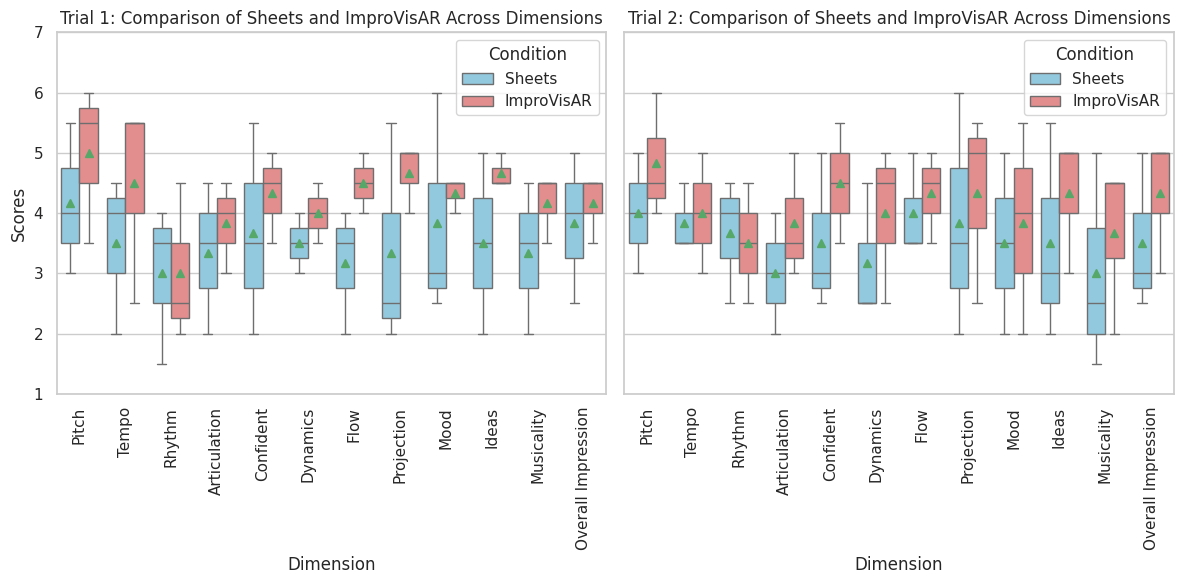
\includegraphics[width=\textwidth]{figs/raterplots.png}
  \caption{%
  	Expert ratings of perceived quality for all the recordings (Trial 1 and Trial 2) comparing those who use each system. %
  }
  \label{fig:expertratings}
\end{figure*}

\par Two (2, 1M, 1F) piano experts were recruited (both are professional piano teachers with 26 years experience on average) in order to gain qualitative review of the performance recordings of the participants during the pilot study. %We expected that experts would rate recordings of \textit{ImproVisAR} learners higher than that of the Sheets system on several dimensions and on overall impression.

\subsubsection{Method and Material}

\par %We recorded one practice (Trial 1) and one actual performance (Trial 2) resulting in 12 recordings (6 recordings from 3 participants who used the \textit{ImproVisAR} system and another 6 recordings from 3 participants who used the Sheets system). Each expert listened to all 12 recordings and filled out a survey for each. Recordings were anonymised and experts did not know which condition was the recording from. They were all presented in randomised order to avoid fatigue and assimilation effects. 
We recorded one practice session (Trial 1) and one actual performance (Trial 2) for each participant, resulting in a total of 12 recordings: 6 from 3 participants using the \textit{ImproVisAR} system and 6 from 3 participants using the Sheets system. Each expert reviewed all 12 recordings and completed a survey for each. To ensure unbiased evaluation, the recordings were anonymised, and the experts were unaware of which system each recording came from. The recordings were presented in random order. % to prevent fatigue and avoid assimilation effects.
%The rating criteria were based on a subset from a music performance adjudication set created by ~\cite{wrigley2013ecological}. We selected the dimensions which are more relevant for improvisation (as the work of ~\cite{rogers2014piano} were focused more on piano playing alone). These dimensions consisted of \textit{pitch, tempo, rhythm, articulation, confidence, dynamics, flow, projection, mood, ideas, musicality} and \textit{overall impression}. Each criterion were on a 7-point Likert scale (from very poor to very good). The experts were also asked to comment on some of their performances. 
The evaluation criteria were based on a subset from a music performance adjudication framework developed by~\cite{wrigley2013ecological}. We selected criteria specifically relevant to improvisation, in contrast to~\cite{rogers2014piano}, which focused more on traditional piano performance. The criteria included \textit{pitch, tempo, rhythm, articulation, confidence, dynamics, flow, projection, mood, ideas, musicality}, and \textit{overall impression}. Each criterion was rated on a 7-point Likert scale (ranging from very poor to very good). Experts were also invited to provide comments on the performances.

\subsubsection{Results and Discussion}

% same dimensions from Rogers : pitch, tempo, articulation, dynamics ONLY
\par %The mean of ratings for the Trial 1 and Trial 2 recordings, across both experts, are plotted and shown in \autoref{fig:expertratings}. Since we only had two experts rating for this pilot study, the means of their ratings would suffice and would not require some form of inter-reliability (e.g. Krippendorff's $\alpha$). The ratings from the \textit{ImproVisAR} Trial 1 recordings were rated higher across all dimensions except for \textit{rhythm}. The same remains consistent as for the Trial 2 recordings from \textit{ImproVisAR}. While the ratings of \textit{rhythm} across both systems were the same (and not higher), we believe that this could be due to several reasons such as having lesser experts to rate (not enough variability) or having a smaller set of participants during the study.
The mean ratings for Trial 1 and Trial 2 recordings, assessed by both experts, are shown in \autoref{fig:expertratings}. Given that only two experts evaluated the recordings in this pilot study, their mean ratings are adequate and do not necessitate inter-rater reliability measures (e.g., Krippendorff's $\alpha$). For Trial 1 recordings, \textit{ImproVisAR} received higher ratings across all criteria except for \textit{rhythm}. This trend was also observed in the Trial 2 recordings for \textit{ImproVisAR}. Ratings for \textit{rhythm} were consistent across both systems and did not show improvement. This uniformity may be attributed to the number of experts, the relatively small participant sample, or non-longitudinal nature of the study (which is a norm in all presented augmented piano prototypes).

\par %Our initial findings echo the results of~\cite{rogers2014piano} where the dimensions of \textit{pitch, tempo, articulation,} and \textit{dynamics} were all rated higher as compared to other systems. While their study explored the effects of piano roll visualisation on teaching piano pressing and sight reading, our system focused on using the same piano roll visualisation but focused on teaching piano improvisation. In addition, our experts also confirmed these ratings citing that ``\textit{confidence is hard to score here but as long as the notes were played right}'' which can be reflected as well on the very positive rating on the \textit{pitch} and \textit{confidence} dimensions of the scale. The dimensions of \textit{flow} and \textit{ideas} show some similar trend from the experts where E2 adds ``\textit{you can observe good flow and confidence at the start but most of them end by the latter parts of their recordings}''. Given that participants only had at most two trials, the expert raters observed that they show some good potential and some hint of confidence at the start of their attempts. While there was an obvious cut in their flow, their progression is evidence despite these limited attempts. 
Our initial findings align with the results from~\cite{rogers2014piano}, which also reported higher ratings for \textit{pitch, tempo, articulation}, and \textit{dynamics} compared to other system. While the mentioned study examined the impact of piano roll visualisations on piano playing and sight reading, our system utilised similar visualisations to focus on teaching piano improvisation. Additionally, our experts supported these findings, noting that ``\textit{confidence is challenging to measure here, but as long as the notes were played correctly}'', which is reflected in the positive ratings for \textit{pitch} and \textit{confidence}. The \textit{flow} and \textit{ideas} dimensions showed a similar trend, with Expert 2 commenting that ``\textit{good flow and confidence are evident at the beginning, but there is a noticeable decline in the latter parts of the recordings}.'' Despite participants having only up to two trials, the experts observed that they demonstrated significant potential and initial confidence. Although there was a noticeable drop in flow towards the end, their overall progression was still evident despite the limited practice.

\section{Initial Qualitative Evaluation}

\par %One of the key contributions of \textit{ImproVisAR} lies in its approach to organising and managing piano improvisation lessons. This design is inspired by the provocations and co-design sessions described in \cite{deja2022piano} and \cite{deja2024teach}. To our knowledge, there has been limited exploration into using augmented reality (AR) for teaching piano improvisation. \textit{ImproVisAR} was specifically developed to address this gap. In this initial evaluation, we shift our focus from examining cognitive load and user experience, as explored in the pilot study, to a deeper investigation into how lessons can be structured and curated. This will help us develop a protocol for a longitudinal study aimed at further validating the impact of AR on improvisation education.
One of the main contributions of \textit{ImproVisAR} is its method for organising and delivering piano improvisation lessons. This approach is influenced by the design strategies and collaborative sessions outlined in~\cite{deja2022piano} and~\cite{deja2024teach}. To date, there has been no research into the use of augmented reality (AR) for longitudinal teaching of complex music concepts such as improvisation, which \textit{ImproVisAR} aims to address. In this initial assessment, our focus shifts from evaluating cognitive load and user experience, as done in the pilot study, to a more detailed examination of lesson structuring and curation. This will guide us in creating a protocol for a longitudinal study to further assess the effectiveness of AR in improvisation education.

\subsection{Participant Recruitment and Protocol}

\par %For this initial study, we recruited two (2, 1M, 1F) participants who has prior music experience, has learned jazz and piano (as a second instrument) and with an average of 6 years of experience playing. They were recruited to a participate in two-hour sessions each, where the goal is to be exposed to all the lessons and all modes in progressive order that was prescribed by one of our expert collaborators. Specifically they will try Lesson 01, then Lesson 02 and Lesson 03 in \texttt{Watch-and-Listen} mode, \texttt{Try Yourself} mode then \texttt{Test Yourself} mode. Then they will try Lesson 04 and Lesson 05 in \texttt{Watch-and-Listen} mode, \texttt{Try Yourself} mode and then followed by \texttt{Compose-On-The-Fly} mode. For this specific mode, they will be given the same Variations and Questions and Answers as described in \autoref{subsec: lessons} where the first half of the lesson (4 out of 8 bars in Lesson 04 and 2 out of 4 bars in Lesson 05) are given while the second half are empty and marked for improvisation (in the sheets displayed). This ``encourages'' the participants to try to improvise given a starting melody. Each lesson has 8 sub-tasks that they all have to watch, then try and then compose, in order. Anytime during the session, they were invited to think-out-aloud and share their insights. During the \texttt{Compose-On-The-Fly} mode, their performances were recorded as well. 
For this initial study, we recruited two participants (2, 1M, 1F) with prior music experience, specifically in jazz and piano (the latter as a secondary instrument), and an average of six years of playing experience. Each participant took part in two-hour sessions designed to expose them to all the lessons and modes in a sequential order as specified by one of our experts. Participants began with Lesson 01, followed by Lesson 02 and Lesson 03, using \texttt{Watch-and-Listen}, \texttt{Try Yourself}, and \texttt{Test Yourself} modes. They then progressed to Lesson 04 and Lesson 05, first in \texttt{Watch-and-Listen} and \texttt{Try Yourself} modes, before moving on to \texttt{Compose-On-The-Fly} mode. In this mode, participants were provided with the Variations and Questions and Answers as outlined in \autoref{subsec: lessons}. For Lesson 04, they received the first 4 out of 8 bars, and for Lesson 05, the first 2 out of 4 bars, with the remainder left blank for improvisation. This setup aimed to encourage participants to improvise starting from a given melody. Each lesson included 8 sub-tasks, which participants were required to follow in sequence: \texttt{Watch-and-Listen}, \texttt{Try Yourself}, and \texttt{Test Yourself}. Throughout the sessions, they were encouraged to think aloud and share their thoughts. Their performances during \texttt{Compose-On-The-Fly} mode were also recorded.

\subsection{Findings and Discussion}

\begin{figure}[tb]% specify a combination of t, b, p, or h for top, bottom, on its own page, or here
  \centering % avoid the use of \begin{center}...\end{center} and use \centering instead (more compact)
  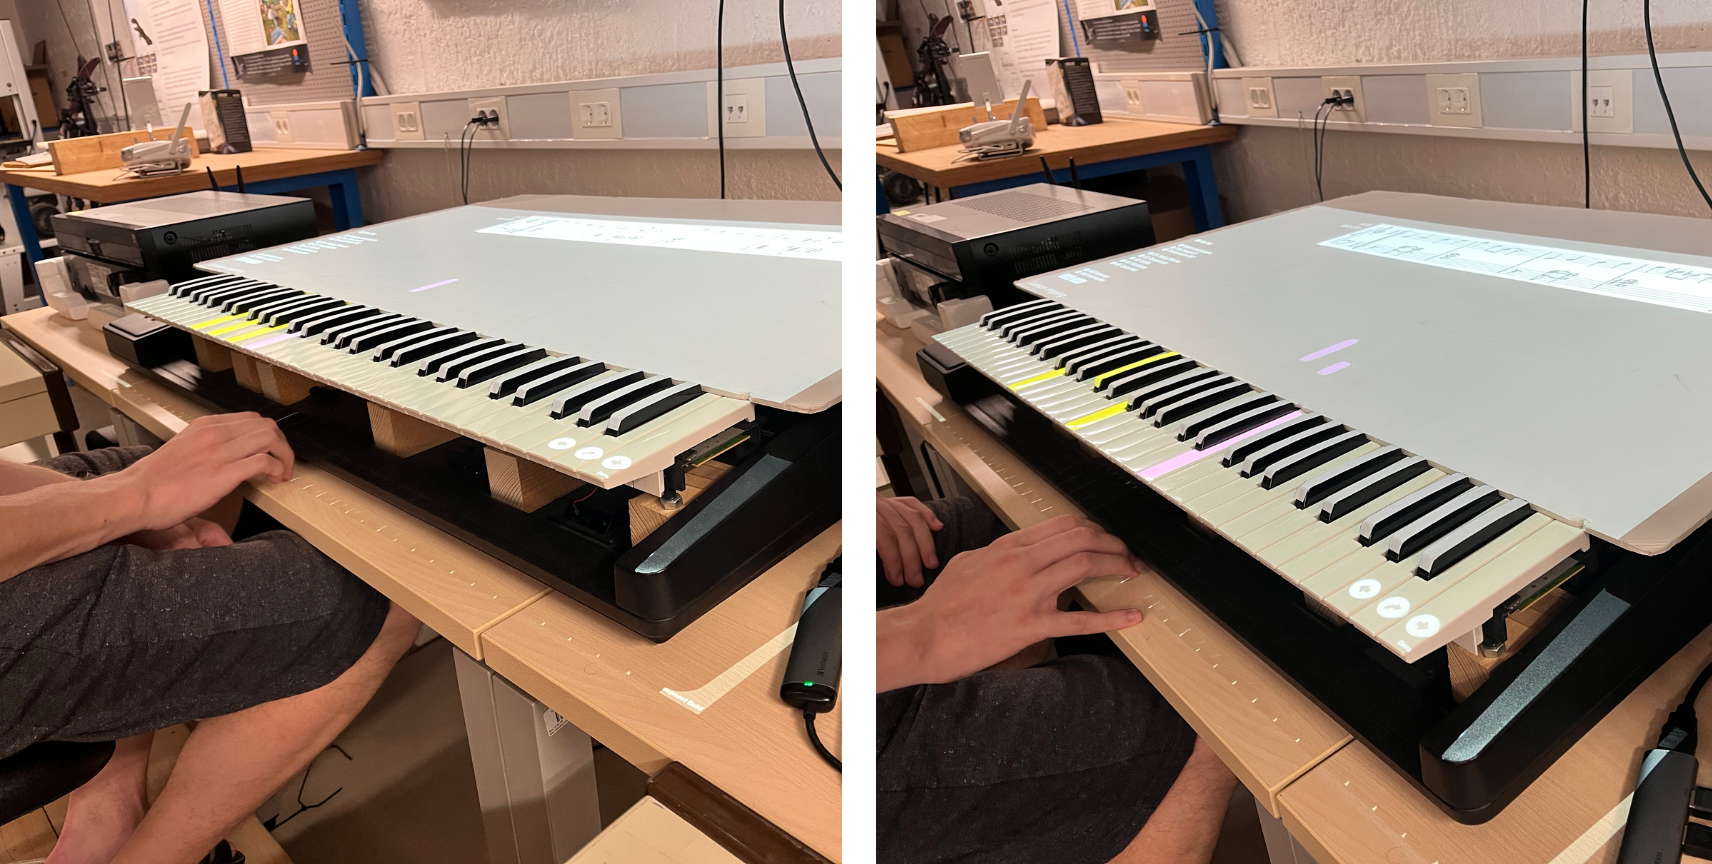
\includegraphics[width=\columnwidth]{figs/shadowing.png}
  \caption{%
  P02, during \texttt{Watch-and-Listen} mode where they are shown practising the chord before proceeding to \texttt{Try Yourself} mode. During this part, they report that they were focused on the falling piano bars while watching and listening. %
  }
  \label{fig:shadowing}
\end{figure}

\par %Based on the qualitative insights of this initial study, both P01 and P02 enjoyed doing \textit{Lesson 01: Swing across all modes}. They treated it as a warm-up for their fingers with P02 adding ``\textit{it's a good way to get refreshed especially if you have not touched the piano in a long time}''. Generally, both participants breezed through most of the earlier lessons in the \textit{ImproVisAR} until the latter part of\textit{ Lesson 03: Motifs}. Both participants reported that the first subtasks (1 to 4) of \textit{Lessons 03-05 (Motifs, Variations and Ques-Ans)} were doable and easy to follow. However, they reported that the latter subtasks (5 to 8) were considered to be too complicated or hard to follow. P01 finds most of these melodies had big jumps which they think would need more practice, while P02 got overwhelmed by the triplets\footnote{A triplet is a rhythm playing three notes in the space of two.} in these melodies. These types of difficulties were earlier reported in the study of ~\cite{giomi2004not} where learners may feel frustrated in trying out some complex music elements (e.g. triplets). Throughout these lessons, the \texttt{Watch-and-Listen} mode were very helpful and some of them had to repeat the lesson several times. P02 (as seen in \autoref{fig:shadowing}) reported that during \texttt{Watch-and-Listen} and prior to \texttt{Try Yourself}, he had to practice and ``shadow'' the position of the keys before they actually try the melodies outside of the piano. These observations were similar to the findings in the work of ~\cite{sloboda1992transitions}. An interesting observation among both participants is that even though they were both comfortable reading music sheets, the experience made them focus on the falling piano bars - and the timely lighting of the keys were of big help in pressing the right keys. These findings concur with the observations on how falling piano bar visualisations help pianists and learners map complex sheet notation and correct finger pressing ~\cite{takegawa2012piano, fernandez2016piano, rogers2014piano}. P01 adds that ``\textit{the falling piano bars were easier to read and while actually playing, I just play by heart after having a quick glimpse at the sheets}''.  
Based on the qualitative feedback from this initial study, both participants (P01 and P02) enjoyed \textit{Lesson 01: Swing} across all modes, viewing it as a finger warm-up exercise. P02 specifically mentioned, ``\textit{it's a good way to get refreshed, especially if you haven't played the piano in a while}''. Both participants found the earlier lessons in \textit{ImproVisAR} relatively easy, but encountered difficulties with the latter parts of \textit{Lesson 03: Motifs}. They reported that the initial sub-tasks (1 to 4) in \textit{Lessons 03-05 (Motifs, Variations, and Question and Answer)} were manageable and straightforward, but the later sub-tasks (5 to 8) were more challenging and complex. P01 noted that the melodies had significant jumps, requiring more practice, while P02 felt overwhelmed by the triplets, a rhythm involving three notes played in the space of two. These difficulties are consistent with previous findings, such as those in~\cite{giomi2004not}, where learners experience frustration with complex musical elements like triplets. The \texttt{Watch-and-Listen} mode was particularly beneficial, with participants repeating the lessons multiple times. P02, for example, reported practising and ``shadowing'' the key positions before attempting the melodies on their own, similar to the observations in~\cite{sloboda1992transitions}. Interestingly, despite both participants being comfortable with reading music sheets, they found the falling piano bars and timed key lighting extremely helpful for pressing the correct keys. This aligns with previous research on how falling piano bar visualisations aid in mapping complex sheet music and improving finger accuracy~\cite{takegawa2012piano, fernandez2016piano, rogers2014piano}. P01 remarked, ``\textit{the falling piano bars were easier to read, and while playing, I just relied on my memory after a quick look at the sheets}''. This result is encouraging and shows that the piano roll visualisation can be beneficial for complex music concepts to advanced learners as well. This also provides a solid foundation for a longitudinal study using our system. 

\par %Even though the latter tasks (5 to 8) of Lessons 03 to 05 were reported to be difficult by both pilot participants, they both had a similar experience during \texttt{Compose-on-the-Fly} mode for Lessons 04 and 05. They did not have to copy a given melody but rather they had to try their best to retain the same core melody (or  same chord tone for Ques-Ans). Both participants felt more fun and less pressure when composing on the fly as this gave them more freedom to play on the spot. These findings were similar to how the study of ~\cite{jutras2006benefits} reports on the effects of fun learning experiences as a key player in piano learning. P02 adds ``\textit{I simply have to follow the chords and stay in the core variation without having to do a triplet or not}''. Both participants believe that rolling piano bars were very helpful especially in making the big jumps in between the key presses. The lessons also helped them ``\textit{know where to start}'' especially when making sure that their improvisationwas within the acceptable and coherent variation.
Despite finding tasks 5 to 8 in Lessons 03 to 05 challenging, both participants had a similar experience with \texttt{Compose-on-the-Fly} mode in Lessons 04 and 05. Instead of replicating a given melody, they focused on maintaining the core melody or chord tones (for Question and Answer). They both enjoyed composing on the fly, finding it more enjoyable and less stressful as it allowed for more spontaneous play. This aligns with findings from~\cite{jutras2006benefits}, which highlight the importance of enjoyable learning experiences in piano education. P02 noted, ``\textit{I just need to follow the chords and stay within the core variation, without worrying about triplets or other complexities}''. Both participants appreciated the falling piano bars for assisting with large jumps between key presses and felt the lessons helped them ``\textit{know where to start}'' and ensure their improvisation stayed within an acceptable and coherent variation.

\par %Being exposed to all the lessons and modes in \textit{ImproVisAR} allowed us to understand whether the presented forms of visualisations were helpful and somehow effective. We had a glimpse of which lessons (or subtasks) would benefit from longer practice sessions (read: more \texttt{Watch-and-Listen} or repetitions across multiple days) especially if we are considering designing the protocol for a longitudinal study. While the findings from this qualitative show some merit, we consider other variables that will help us understand the effects of prolonged exposure to piano roll visualisations (e.g. subjective cognitive load, flow state and creativity support and many others, eye tracking and its analysis). 
Exposing participants to all the lessons and modes in \textit{ImproVisAR} provided insights into the effectiveness of the visualisations and their utility. It highlighted which lessons or sub-tasks might benefit from extended practice sessions, such as additional \texttt{Watch-and-Listen} sessions or repeated practice over multiple days, especially when planning a longitudinal study. Although this qualitative analysis reveals some promising aspects, further investigation is needed into additional factors, such as subjective cognitive load, flow state, creativity support, and eye tracking, to better understand the impact of prolonged use of piano roll visualisations.


% \par in terms of cognitive load, demand experienced by participants during the task 1 and task 2 are both lower for \textit{ImproVisAR} as compared to the other system. this echoes the findings of rogers. 


% 
% \par expert ratings echo that of the work of ~\cite{rogers2014piano} where the use of augmentation have better pitch, tempo, and dynamics. However, some criteria were opposite to that of their findings such as in articulation, rhythm and overall impression. 



% \subsection{On Protocol and Lesson Sequence}

% \subsection{On Findings}


\section{Conclusion and Future Work}
\par In this paper, we presented \textit{ImproVisAR}, an augmented reality training system that leverages piano roll visualisations to teach piano improvisation. Its modes and lessons were inspired by the best features identified in a survey of augmented piano prototypes in educational contexts
%~\cite{deja2022survey}, 
as well as insights from a co-design process with piano improvisation teaching experts.
%\cite{deja2024teach}. 
What distinguishes our system from previous piano roll prototypes is that our system incorporated the whole training process with a focus on teaching complex music concepts to advanced piano player. For this reason we designed the system and visualisations in the iterative process with music experts and piano player, as well as adapted the visualisations accordingly. 
In this paper we describe the system’s features and conducted a pilot study with $n=6$ participants, assessing subjective cognitive load, perceived user experience, and preferences compared to the traditional music sheet condition. The findings from a pilot study using a small subset of lessons suggest a positive acceptance of the visualisation, but they also highlight the need for further investigation. We also conducted the initial study using entire learning content with $n=2$ participants, who experienced the prototype in a more intimate, structured sessions exploring all lessons and modes. The insights from this study informed the design of a more controlled longitudinal study aimed at thoroughly assessing the effectiveness of augmented piano roll visualisations in teaching complex music concepts such as improvisation. %We encourage future work to build on these discussions, considering factors such as learner performance evaluation, creativity support, flow state measurement, and more.

%an experimental protocol involving a longitudinal study in a controlled setup 

%While the findings are inconclusive, they denote some potential that calls for a longitudinal study, in a controlled setup evaluating its effectiveness  in teaching jazz piano improvisation. The current features and lessons of the systems merits a proper evaluation considering several factors such as, length of the program, arrangement and grouping of lessons and a considering other variables such as evaluating performance, creativity support, flow state and many others. 

%====== any below this will be commented out. do not delete latex code for code reference ======== 

% \section{Author Details}

% You should specify ORCID IDs for each author (see \url{https://orcid.org/}  to register) for disambiguation and long-term contact preservation.
% Use \verb|\authororcid{Author Name}{0000-0000-0000-0000}| for each author, replacing the ``Author Name'' and using the 16-digit (hyphenated) ORCID ID for the second parameter.
% The template shows an example without ORCID IDs for two of the authors.
% ORCID IDs should be provided in all cases.

% Each author's affiliations have to be provided in the author footer on the bottom-left corner of the first page.
% It is permitted to merge two or more people from the same institution as long as they are shown in the same order as in the overall author sequence on the top of the first page.
% For example, if authors A, B, C, and D are from institutions 1, 2, 1, and 2, respectively, then it is ok to use 2 bullets as follows:
% \begin{itemize}
%   \item A and C are with Institution 1. E-mail: \{a\,$|$\,c\}@i1.com\,.

%   \item B and D are with Institution 2. E-mail: \{b\,$|$\,d\}@i2.org\,.
% \end{itemize}


% \section{Hyperlinks and Cross References}

% The style uses the \verb|hyperref| package which can typeset clickable hyperlinks using \verb|\href{...}{...}|, hyperlinked URLs using \verb|\url{...}|, and turns references into internal links.

% The style also uses \verb|cleveref| to automatically and consistently format cross references.
% We recommend that you use the \verb|\cref{label}| and \verb|\Cref{label}| calls instead of \verb|Figure~\ref{label}| or similar.
% \verb|\Cref| should be used when starting a sentence to spell out the reference (e.g.\ ``Section'') while \verb|\cref| should be used when referencing within a sentence to abbreviate (e.g.\ ``Sec.'').
% Here are examples for use within a sentence: \cref{fig:vis_papers}, \cref{tab:vis_papers}, \cref{sec:supplement_inst,sec:references_inst}, \cref{eq:sum}.
% The following sentences all start with a reference, so use \verb|\Cref|.
% \Cref{fig:vis_papers} is a \verb|figure| environment.
% \Cref{tab:vis_papers} is a \verb|table| environment.
% \Cref{sec:supplement_inst,sec:references_inst} are \verb|section| environments.
% \Cref{eq:sum} is an \verb|equation| environment.


% \section{Figures}

% \subsection{Loading figures}

% The style automatically looks for image files with the correct extension (eps for regular \LaTeX; pdf, png, and jpg for pdf\LaTeX), in a set of given subfolders defined above using \verb|\graphicspath|: figures/, pictures/, images/.
% It is thus sufficient to use \verb|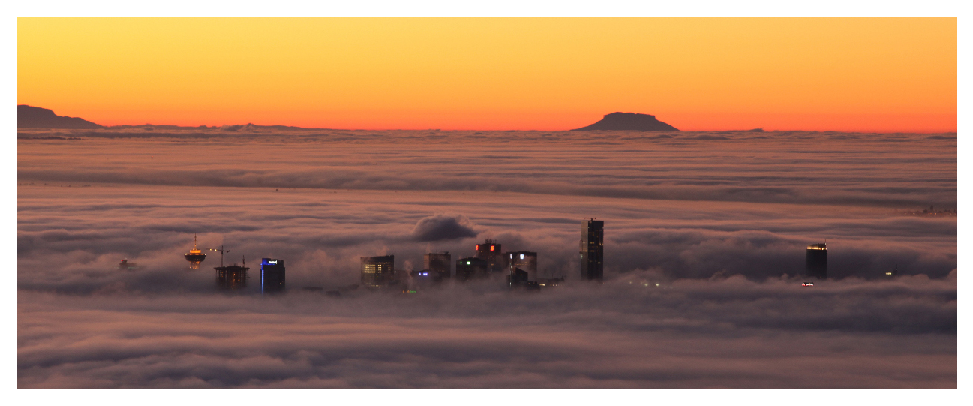
\includegraphics{CypressView}| (instead of \verb|\includegraphics{pictures/CypressView.jpg}|).
% Figures should be in CMYK or Grey scale format, otherwise, colour shifting may occur during the printing process.

% \subsection{Vector figures}

% Vector graphics like svg, eps, pdf are best for charts and other figures with text or lines.
% They will look much nicer and crisper and any text in them will be more selectable, searchable, and accessible.

% \subsection{Raster figures}

% Of the raster graphics formats, screenshots of user interfaces and text, as well as line art, are better shown with png.
% jpg is better for photographs.
% Make sure all raster graphics are captured in high enough resolution so they look crisp and scale well.

% \subsection{Figures on the first page}

% The teaser figure should only have the width of the abstract as the template enforces it.
% The use of figures other than the optional teaser is not permitted on the first page.
% Other figures should begin on the second page.
% Papers submitted with figures other than the optional teaser on the first page will be refused.

% \subsection{Subfigures}

% You can add subfigures using the \texttt{subcaption} package that is automatically loaded.
% Inside a \verb|figure| environment, create a \verb|subfigure| environment.
% See \cref{fig:ex_subfigs} for an example.
% You can reference individual figures, either fully using \verb|\cref| (\cref{fig:ex_subfigs_a,fig:ex_subfigs_b}) or by letter using \verb|\subref|.
% E.g., \subref{fig:ex_subfigs_b}, \subref{fig:ex_subfigs_c}.
% Note that \verb|\subref| only works for one label at a time.

% \begin{figure}[tbp]
%   \centering
%   \begin{subfigure}[b]{0.45\columnwidth}
%   	\centering
%   	\includegraphics[width=\textwidth]{example-image-a}
%   	\caption{The letter A.}
%   	\label{fig:ex_subfigs_a}
%   \end{subfigure}%
%   \hfill%
%   \begin{subfigure}[b]{0.45\columnwidth}
%   	\centering
%   	\includegraphics[width=\textwidth]{example-image-b}
%   	\caption{The letter B.}
%   	\label{fig:ex_subfigs_b}
%   \end{subfigure}%
%   \\%
%   \begin{subfigure}[b]{0.45\columnwidth}
%   	\centering
%   	\includegraphics[width=\textwidth]{example-image-c}
%   	\caption{The letter C.}
%   	\label{fig:ex_subfigs_c}
%   \end{subfigure}%
%   \subfigsCaption{Example of adding subfigures with the \texttt{subcaption} package.}
%   \label{fig:ex_subfigs}
% \end{figure}

% \subsection{Figure Credits}
% \label{sec:figure_credits_inst}

% In the \hyperref[sec:figure_credits]{Figure Credits} section at the end of the paper, you should credit the original sources of any figures that were reproduced or modified.
% Include any license details necessary, as well as links to the original materials whenever possible.
% For credits to figures from academic papers, include a citation that is listed in the \textbf{References} section.
% An example is provided \hyperref[sec:figure_credits]{below}.


% \section{Equations and Tables}

% Equations can be added like so:

% \begin{equation}
%   \label{eq:sum}
%   \sum_{j=1}^{z} j = \frac{z(z+1)}{2}
% \end{equation}

% Tables, such as \cref{tab:vis_papers} can also be included.


% \begin{table}[tb]
%   \caption{%
%   	VIS/VisWeek accepted/presented papers: 1990--2016.%
%   }
%   \label{tab:vis_papers}
%   \scriptsize%
%   \centering%
%   \begin{tabu}{%
%   	  r%
%   	  	*{7}{c}%
%   	  	*{2}{r}%
%   	}
%   	\toprule
%   	year & \rotatebox{90}{Vis/SciVis} &   \rotatebox{90}{SciVis conf} &   \rotatebox{90}{InfoVis} &   \rotatebox{90}{VAST} &   \rotatebox{90}{VAST conf} &   \rotatebox{90}{TVCG @ VIS} &   \rotatebox{90}{CG\&A @ VIS} &   \rotatebox{90}{VIS/VisWeek} \rotatebox{90}{incl.\ TVCG/CG\&A}   &   \rotatebox{90}{VIS/VisWeek} \rotatebox{90}{w/o TVCG/CG\&A}   \\
%   	\midrule
%   	2016 & 30 &   & 37 & 33 & 15 & 23 & 10 & 148 & 115 \\
%   	2015 & 33 & 9 & 38 & 33 & 14 & 17 & 15 & 159 & 127 \\
%   	2014 & 34 &   & 45 & 33 & 21 & 20 &    & 153 & 133 \\
%   	2013 & 31 &   & 38 & 32 &    & 20 &    & 121 & 101 \\
%   	2012 & 42 &   & 44 & 30 &    & 23 &    & 139 & 116 \\
%   	2011 & 49 &   & 44 & 26 &    & 20 &    & 139 & 119 \\
%   	2010 & 48 &   & 35 & 26 &    &    &    & 109 & 109 \\
%   	2009 & 54 &   & 37 & 26 &    &    &    & 117 & 117 \\
%   	2008 & 50 &   & 28 & 21 &    &    &    &  99 &  99 \\
%   	2007 & 56 &   & 27 & 24 &    &    &    & 107 & 107 \\
%   	2006 & 63 &   & 24 & 26 &    &    &    & 113 & 113 \\
%   	2005 & 88 &   & 31 &    &    &    &    & 119 & 119 \\
%   	2004 & 70 &   & 27 &    &    &    &    &  97 &  97 \\
%   	2003 & 74 &   & 29 &    &    &    &    & 103 & 103 \\
%   	2002 & 78 &   & 23 &    &    &    &    & 101 & 101 \\
%   	2001 & 74 &   & 22 &    &    &    &    &  96 &  96 \\
%   	2000 & 73 &   & 20 &    &    &    &    &  93 &  93 \\
%   	1999 & 69 &   & 19 &    &    &    &    &  88 &  88 \\
%   	1998 & 72 &   & 18 &    &    &    &    &  90 &  90 \\
%   	1997 & 72 &   & 16 &    &    &    &    &  88 &  88 \\
%   	1996 & 65 &   & 12 &    &    &    &    &  77 &  77 \\
%   	1995 & 56 &   & 18 &    &    &    &    &  74 &  74 \\
%   	1994 & 53 &   &    &    &    &    &    &  53 &  53 \\
%   	1993 & 55 &   &    &    &    &    &    &  55 &  55 \\
%   	1992 & 53 &   &    &    &    &    &    &  53 &  53 \\
%   	1991 & 50 &   &    &    &    &    &    &  50 &  50 \\
%   	1990 & 53 &   &    &    &    &    &    &  53 &  53 \\
%   	\midrule               
%   	\textbf{sum} & \textbf{1545} & \textbf{9} & \textbf{632} & \textbf{310} & \textbf{50} & \textbf{123} & \textbf{25} & \textbf{2694} & \textbf{2546} \\
%   	\bottomrule
%   \end{tabu}%
% \end{table}

% \begin{figure}[tb]% specify a combination of t, b, p, or h for top, bottom, on its own page, or here
%   \centering % avoid the use of \begin{center}...\end{center} and use \centering instead (more compact)
%   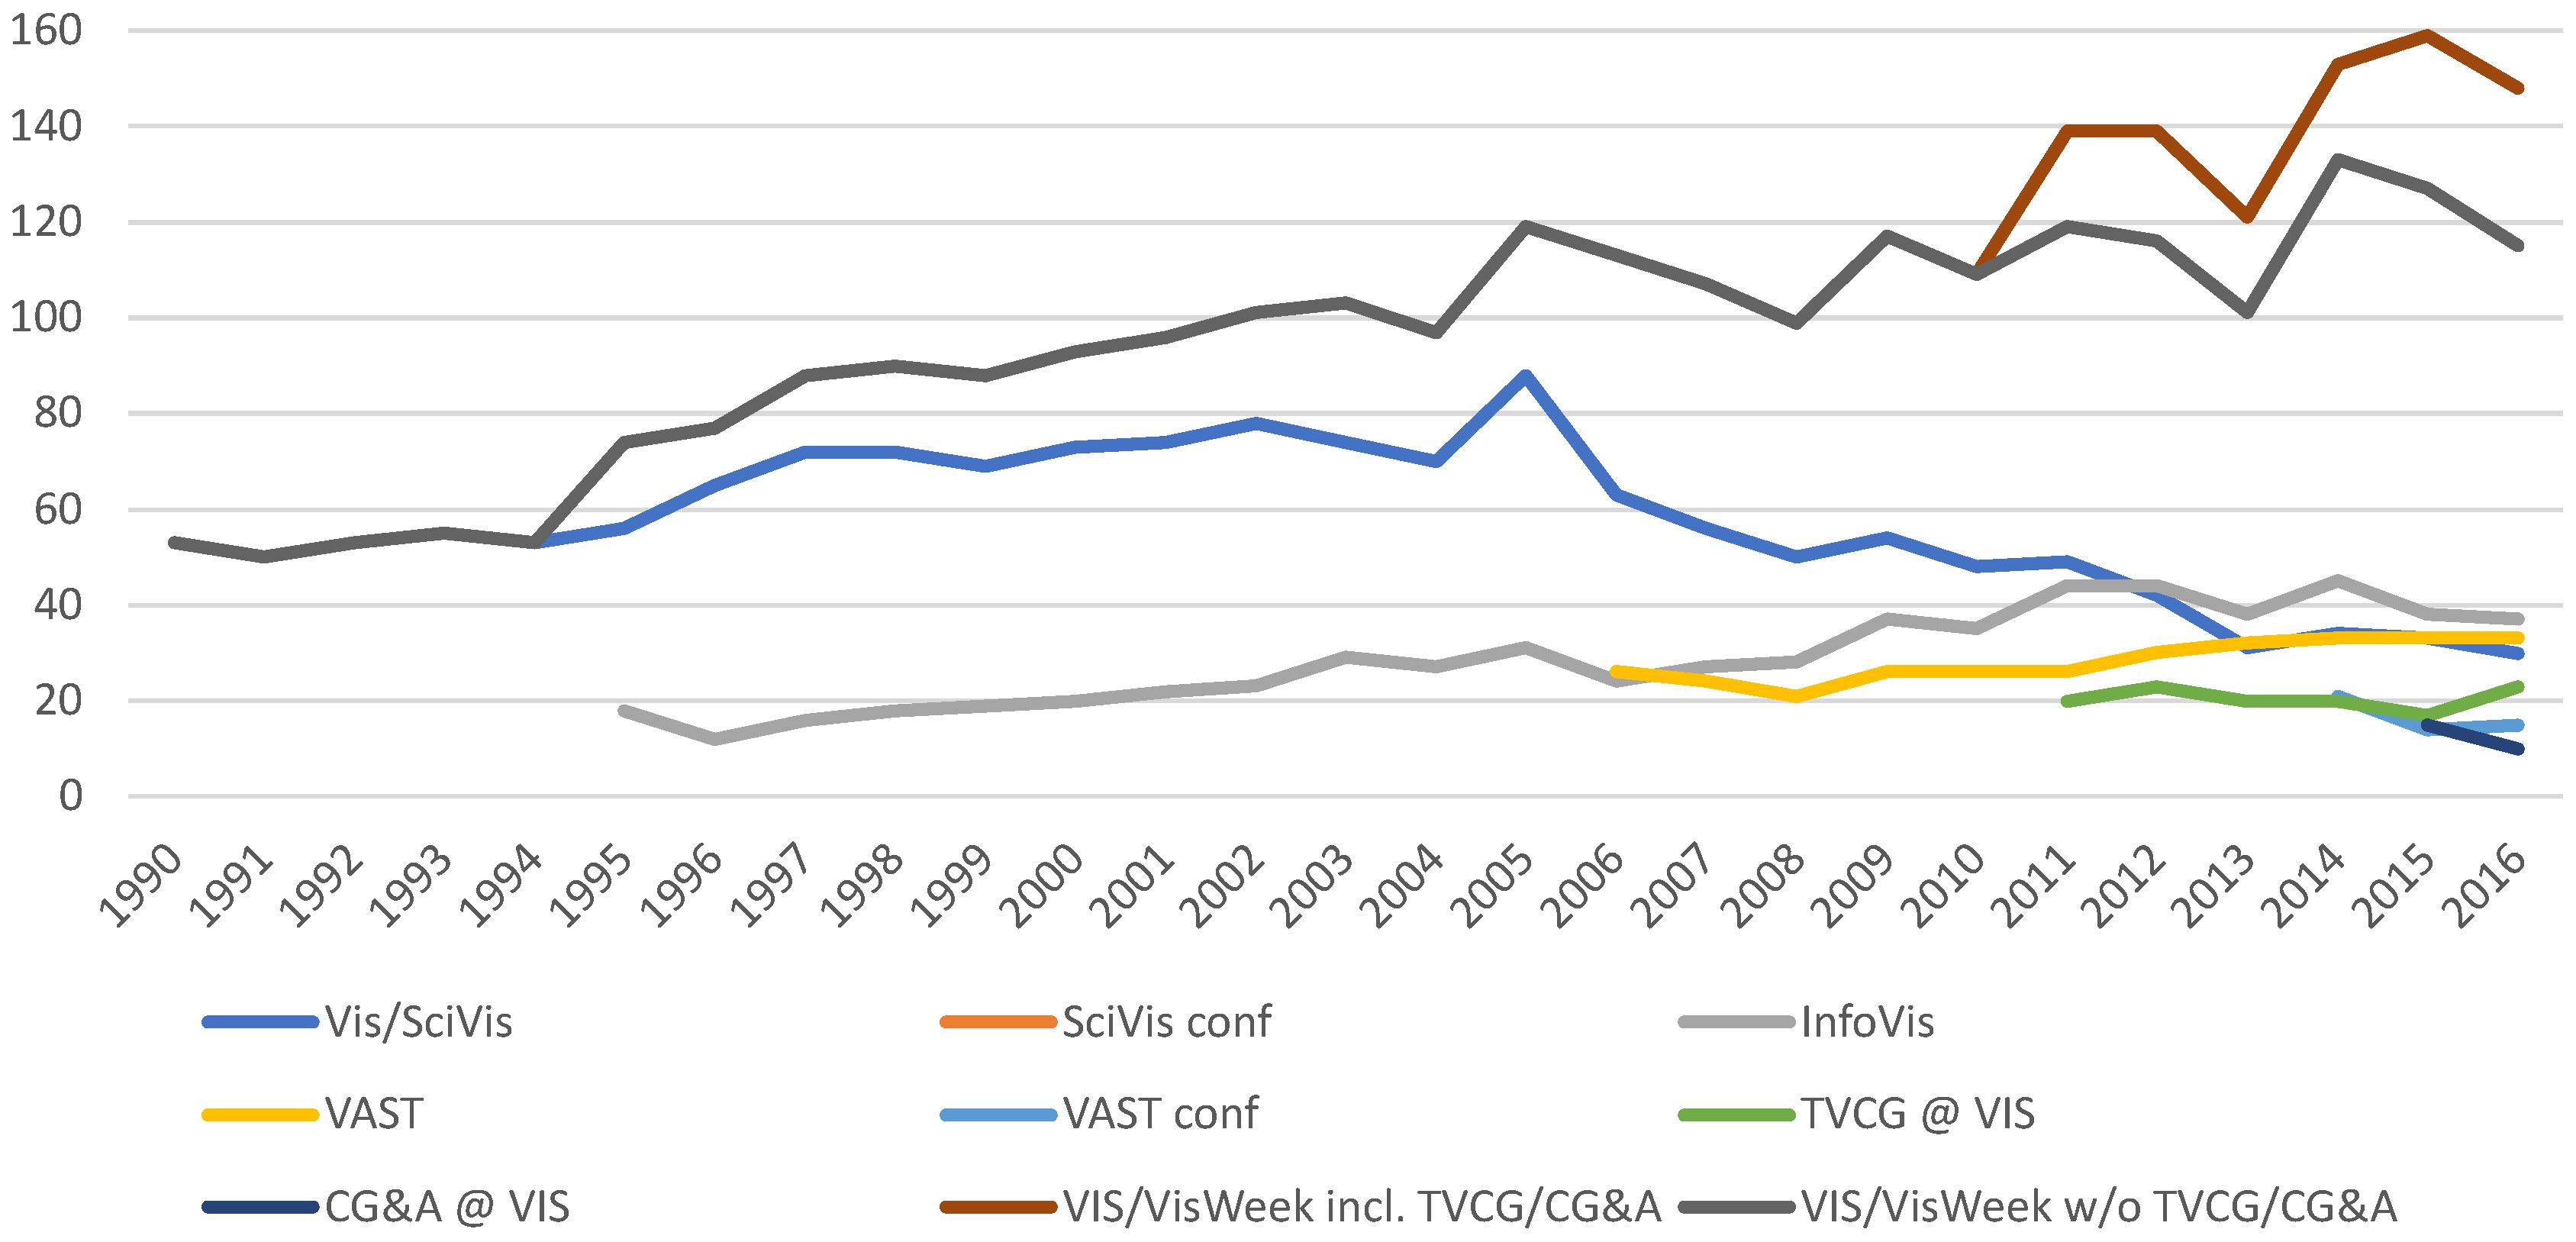
\includegraphics[width=\columnwidth]{paper-count-2016}
%   \caption{%
%   	A visualisation of the 1990--2016 data from \cref{tab:vis_papers}, recreated based on Fig.\ 1 from \cite{Isenberg:2017:VMC}.%
%   }
%   \label{fig:vis_papers}
% \end{figure}


% \section{Supplemental Material Instructions}
% \label{sec:supplement_inst}

% In support of transparent research practices and long-term open science goals, you are encouraged to make your supplemental materials available on a publicly-accessible repository.
% Please describe the available supplemental materials in the \hyperref[sec:supplemental_materials]{Supplemental Materials} section.
% These details could include (1) what materials are available, (2) where they are hosted, and (3) any necessary omissions.


% \section{References}
% \label{sec:references_inst}

% An example of the reference formatting is provided in the \textbf{References} section at the end.


% \subsection{Include DOIs}

% All references which have a DOI should have it included in the bib\TeX\ for the style to display.
% The DOI can be entered with or without the \url{https://doi.org/} prefix.

% \subsection{Narrow DOI option}

% The \verb|-narrow| versions of the bibliography style use the font \verb|PTSansNarrow-TLF| for typesetting the DOIs in a compact way.
% This font needs to be available on your \LaTeX\ system.
% It is part of the \href{https://www.ctan.org/pkg/paratype}{\texttt{paratype} package}, and many distributions (such as MikTeX) have it automatically installed.
% If you do not have this package yet and want to use a \verb|-narrow| bibliography style then use your \LaTeX\ system's package installer to add it.
% If this is not possible you can also revert to the respective bibliography styles without the \verb|-narrow| in the file name.
% DVI-based processes to compile the template apparently cannot handle the different font so, by default, the template file uses the \texttt{abbrv-doi} bibliography style.

% \subsection{Disabling hyperlinks}

% To avoid adding hyperlinks to the references (the default) you can use \verb|\bibliographystyle{abbrv-doi}| instead of \verb|\bibliographystyle{abbrv-doi-hyperref}|.
% By default, the DOI field in a bib\TeX\ entry is turned into a hyperlink.

% See the examples in the bib\TeX\ file and the bibliography at the end of this template.

% \subsection{Guidelines for bibTeX}

% \begin{itemize}
%   \item All bibliographic entries should be sorted alphabetically by the last name of the first author.
%         This \LaTeX/bib\TeX\ template takes care of this sorting automatically.
%   \item Merge multiple references into one; e.\,g., use \cite{Max:1995:OMF,Kitware:2003} (not \cite{Kitware:2003}\cite{Max:1995:OMF}).
%         Within each set of multiple references, the references should be sorted in ascending order.
%         This \LaTeX/bib\TeX\ template takes care of both the merging and the sorting automatically.
%   \item Verify all data obtained from digital libraries, even ACM's DL and IEEE Xplore  etc.\ are sometimes wrong or incomplete.
%   \item Do not trust bibliographic data from other services such as Mendeley.com, Google Scholar, or similar; these are even more likely to be incorrect or incomplete.
%   \item Articles in journal---items to include:
%         \begin{itemize}
%   	      \item author names
%   	      \item title
%   	      \item journal name
%   	      \item year
%   	      \item volume
%   	      \item number
%   	      \item month of publication as variable name (i.e., \{jan\} for January, etc.; month ranges using \{jan \#\{/\}\# feb\} or \{jan \#\{-{}-\}\# feb\})
%         \end{itemize}
%   \item Use journal names in proper style: correct: ``IEEE Transactions on Visualisation and Computer Graphics'', incorrect: ``Visualisation and Computer Graphics, IEEE Transactions on''
%   \item Papers in proceedings---items to include:
%         \begin{itemize}
%   	      \item author names
%   	      \item title
%   	      \item abbreviated proceedings name: e.g., ``Proc.\textbackslash{} CONF\_ACRONYNM'' without the year; example: ``Proc.\textbackslash{} CHI'', ``Proc.\textbackslash{} 3DUI'', ``Proc.\textbackslash{} Eurographics'', ``Proc.\textbackslash{} EuroVis''
%   	      \item year
%   	      \item publisher
%   	      \item town with country of publisher (the town can be abbreviated for well-known towns such as New York or Berlin)
%         \end{itemize}

%   \item Article/paper title convention: refrain from using curly brackets, except for acronyms/proper names/words following dashes/question marks etc.; example:\\\\
%         %
%         The paper ``Marching Cubes: A High Resolution 3D Surface Construction Algorithm'' should be entered as ``\{M\}arching \{C\}ubes: A High Resolution \{3D\} Surface Construction Algorithm'' or  ``\{M\}arching \{C\}ubes: A high resolution \{3D\} surface construction algorithm''.
%         It will then be typeset as ``Marching Cubes: A high resolution 3D surface construction algorithm''
%   \item For all entries:
%         \begin{itemize}
%   	      \item DOI can be entered in the DOI field as plain DOI number or as DOI url.
%   	      \item Provide full page ranges AA-{}-BB
%         \end{itemize}
%   \item When citing references, do not use the reference as a sentence object; e.g., wrong: ``In \cite{Lorensen:1987:MCA} the authors describe \dots'', correct: ``Lorensen and Cline \cite{Lorensen:1987:MCA} describe \dots''
% \end{itemize}

% \section{Appendices}
% \label{sec:appendices_inst}

% Appendices can be specified using \verb|\appendix|.
% For example, our Troubleshooting instructions in
% \iflabelexists{appendix:troubleshooting}
%   {\cref{appendix:troubleshooting}}
%   {the appendix of the full paper at \url{https://osf.io/nrmyc}}.

% Note that the paper submission has to end after the \textbf{References} section and within the page limit of the conference you are submitting to.
% Any version of Appendices or the paper with Appendices included has to be submitted separately as supplementary material.
% You can use the \verb|hideappendix| class option to remove everything after \verb|\appendix|.
% We encourage you to submit a full version of your paper to a preprint server with any appendices included.

% You can use the \verb|\iflabelexists| macro to cross reference an appendix from the main text, but only if that label (i.e.\ the appendix) actually exists.
% For example, above we use 

% \begin{verbatim}
% \iflabelexists{appendix:troubleshooting}
%   {\cref{appendix:troubleshooting}}
%   {the appendix of the full paper at
%    \url{https://osf.io/XXXXX}}.
% \end{verbatim}

% in order to cross-reference to the appendix with \verb|\cref| if it exists, but if the appendix is commented out then we will simply create a hyperlinked URL to it.


% \section{Filler Text to Flush Out the Paper}

% \lipsum[1-2]% Just add some more arbitrary text so we see a fuller paper example


% \section*{Supplemental Materials}
% \label{sec:supplemental_materials}

% Refer to the instructions for this section (\cref{sec:supplement_inst}).
% Below is an example you can follow that includes the actual supplemental material for this template:

% All supplemental materials are available on OSF at \url{https://doi.org/10.17605/OSF.IO/2NBSG}, released under a CC BY 4.0 license.
% In particular, they include (1) Excel files containing the data for and analyses for creating \cref{tab:vis_papers} and \cref{fig:vis_papers}, (2) figure images in multiple formats, and (3) a full version of this paper with all appendices.
% Our other code is intellectual property of a corporation---Starbucks Research---and there is no feasible way to share it publicly.


% \section*{Figure Credits}
% \label{sec:figure_credits}

% Refer to the instructions for this section (\cref{sec:figure_credits_inst}).
% Here are the actual figure credits for this template:

% \Cref{fig:teaser} image credit: Scott Miller / Special to the Vancouver Sun, January 22, 2009, page A6.

% \Cref{fig:vis_papers} is a partial recreation of Fig.\ 1 from \cite{Isenberg:2017:VMC}, which is in the public domain.


%% if specified like this the section will be ommitted in review mode
\acknowledgments{%
	The authors wish to thank A, B, and C.
  This work was supported in part by a grant from XYZ (\# 12345-67890).%
}


%\bibliographystyle{abbrv}
\bibliographystyle{abbrv-doi}
%\bibliographystyle{abbrv-doi-narrow}
%\bibliographystyle{abbrv-doi-hyperref}
%\bibliographystyle{abbrv-doi-hyperref-narrow}

\bibliography{template}
\end{document}
